% !TEX root = ../paper.tex
\section{Interaction techniques} \label{sec:techniques}
In this section we illustrate and describe the interaction techniques we implemented in order to exchange data between mobile phones and large displays.
This is done so that we can compare them to one another empirically.

There were several criteria behind the choice of these techniques. 
\Cref{tab:techniqueCriteria} shows the set of criteria that we based our choice of techniques on.

\begin{table}[H]
	\centering
	\def\arraystretch{1.5}
	\begin{tabular}{p{0.2\columnwidth} p{0.7\columnwidth}}
		\hline
		\textbf{Attributes} & \textbf{Description} \\ \hline
		\textit{Number of hands} & There must be both one-handed and two-handed techniques. \\ \hline
		\textit{Previously used} & To avoid designing and testing a set of novel techniques, we had the criterion that all techniques have been used by others in research studies. \\ \hline
		\textit{Complexity} & The techniques must differ in their complexity and therefore we included techniques with different amount of steps. \\ \hline
		\textit{Activation method} & The way each technique is activated must be different from each other. \\ \hline
		\textit{Natural feel} & There must be a natural and intuitive feel to the techniques in some way. \\ \hline
	\end{tabular}
	\caption{Criteria for selection}
	\label{tab:techniqueCriteria}
\end{table}
%Two-handed techniques which are techniques that require both hands.


The techniques chosen were found in the literature, some with minor modifications.
We then created a symmetrical version of each technique so they would have both a \push and \pull version.
\push means that the user is pushing data from the mobile to the large display, and \pull means the user will pull data from the screen onto the mobile device. 

Eight techniques were used in the experiment: \alltechniques, each with a \push and \pull variant.

\subsubsection{Grab} \label{sec:grabTechnique}
The \grab technique is based on a grabbing gesture presented by Hespanhol et al. \cite{Hespanhol:2012} as one of five proposed gestures.
A related technique is described by Markussen et al. \cite{Markussen:2014}. 
They present a mid-air word-gesture keyboard named \emph{``Vulture''} that uses a pinch gesture (touching index finger to thumb) to give the user control of the pointer which can then be used to select letters.
A variation of the \grab technique (\cref{fig:grabTechnique}) is used in \emph{Memory Stones} \cite{Ikematsu:2015} by Ikemasu et al. as part of a system for exchanging information between different devices. Benko and Wilson \cite{Benko:2010} used the \grab technique in a system where the user interacts with visualizations inside a dome. \grab is a combination of the grabbing gesture and the pointing technique used by Scheible et al. \cite{Scheible:2008}.
This technique was chosen because we wanted to simulate the feeling of picking up an object of interest and placing it in a desired location.
\grab is a complex technique, requiring a series of steps as well as using both hands to complete the interaction.
The \push version of this technique is completed as follows: the user first grabs an object of interest from the telephone by pinching it with his fingers (\cref{fig:grabTechniqueA}), closing his hand, and metaphorically putting the object in his hands.
The user then raises his closed hand and uses it as a pointer on the screen to indicate where he wants to place the object (\cref{fig:grabTechniqueB}).
The final step is to open the hand and release the object onto the large display, where he was aiming (\cref{fig:grabTechniqueC}).
The \pull version is a bit different.
The user first places his open hand, used as a pointer, over the position of the object of interest on the large display (\cref{fig:grabTechniqueC}).
The user then closes his hand over the object (\cref{fig:grabTechniqueB}) and finally places it on his phone by touching the screen with his closed hand (\cref{fig:grabTechniqueB}).  

\begin{figure}[H]
	\subfloat[]{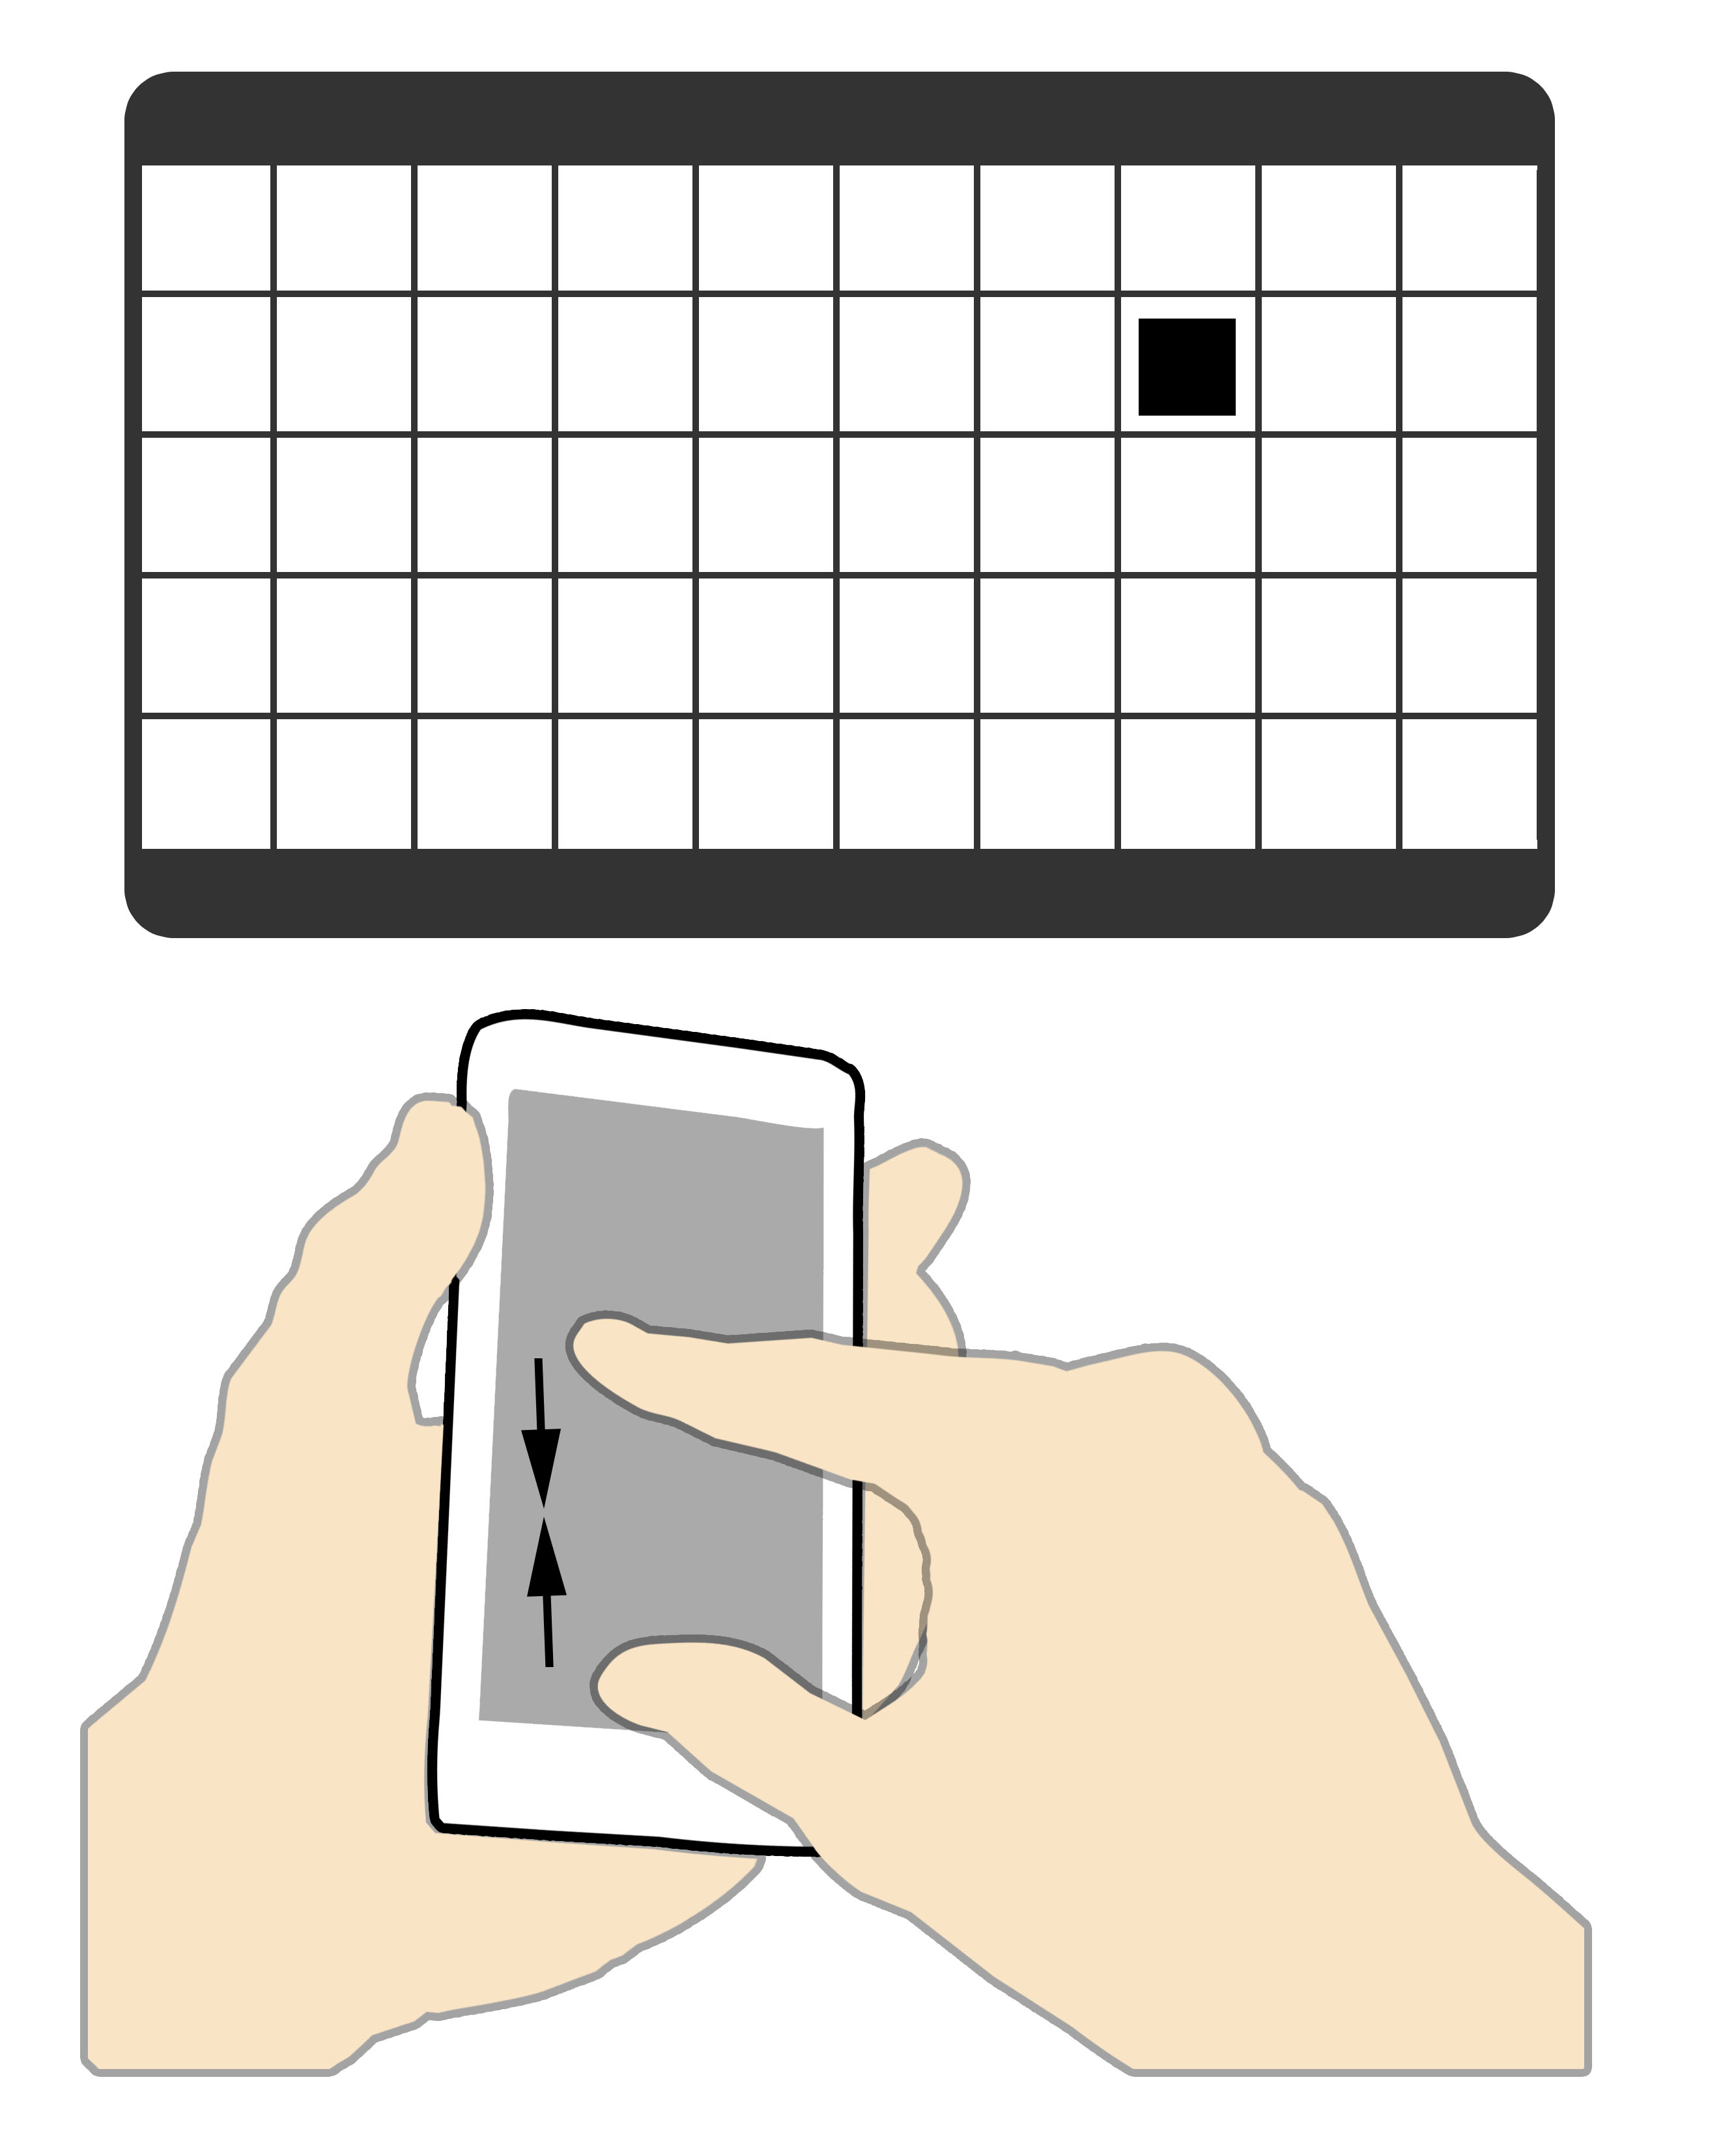
\includegraphics[width = 0.33\columnwidth]{images/techniques/grabPush1.jpg}\label{fig:grabTechniqueA}}
	\subfloat[]{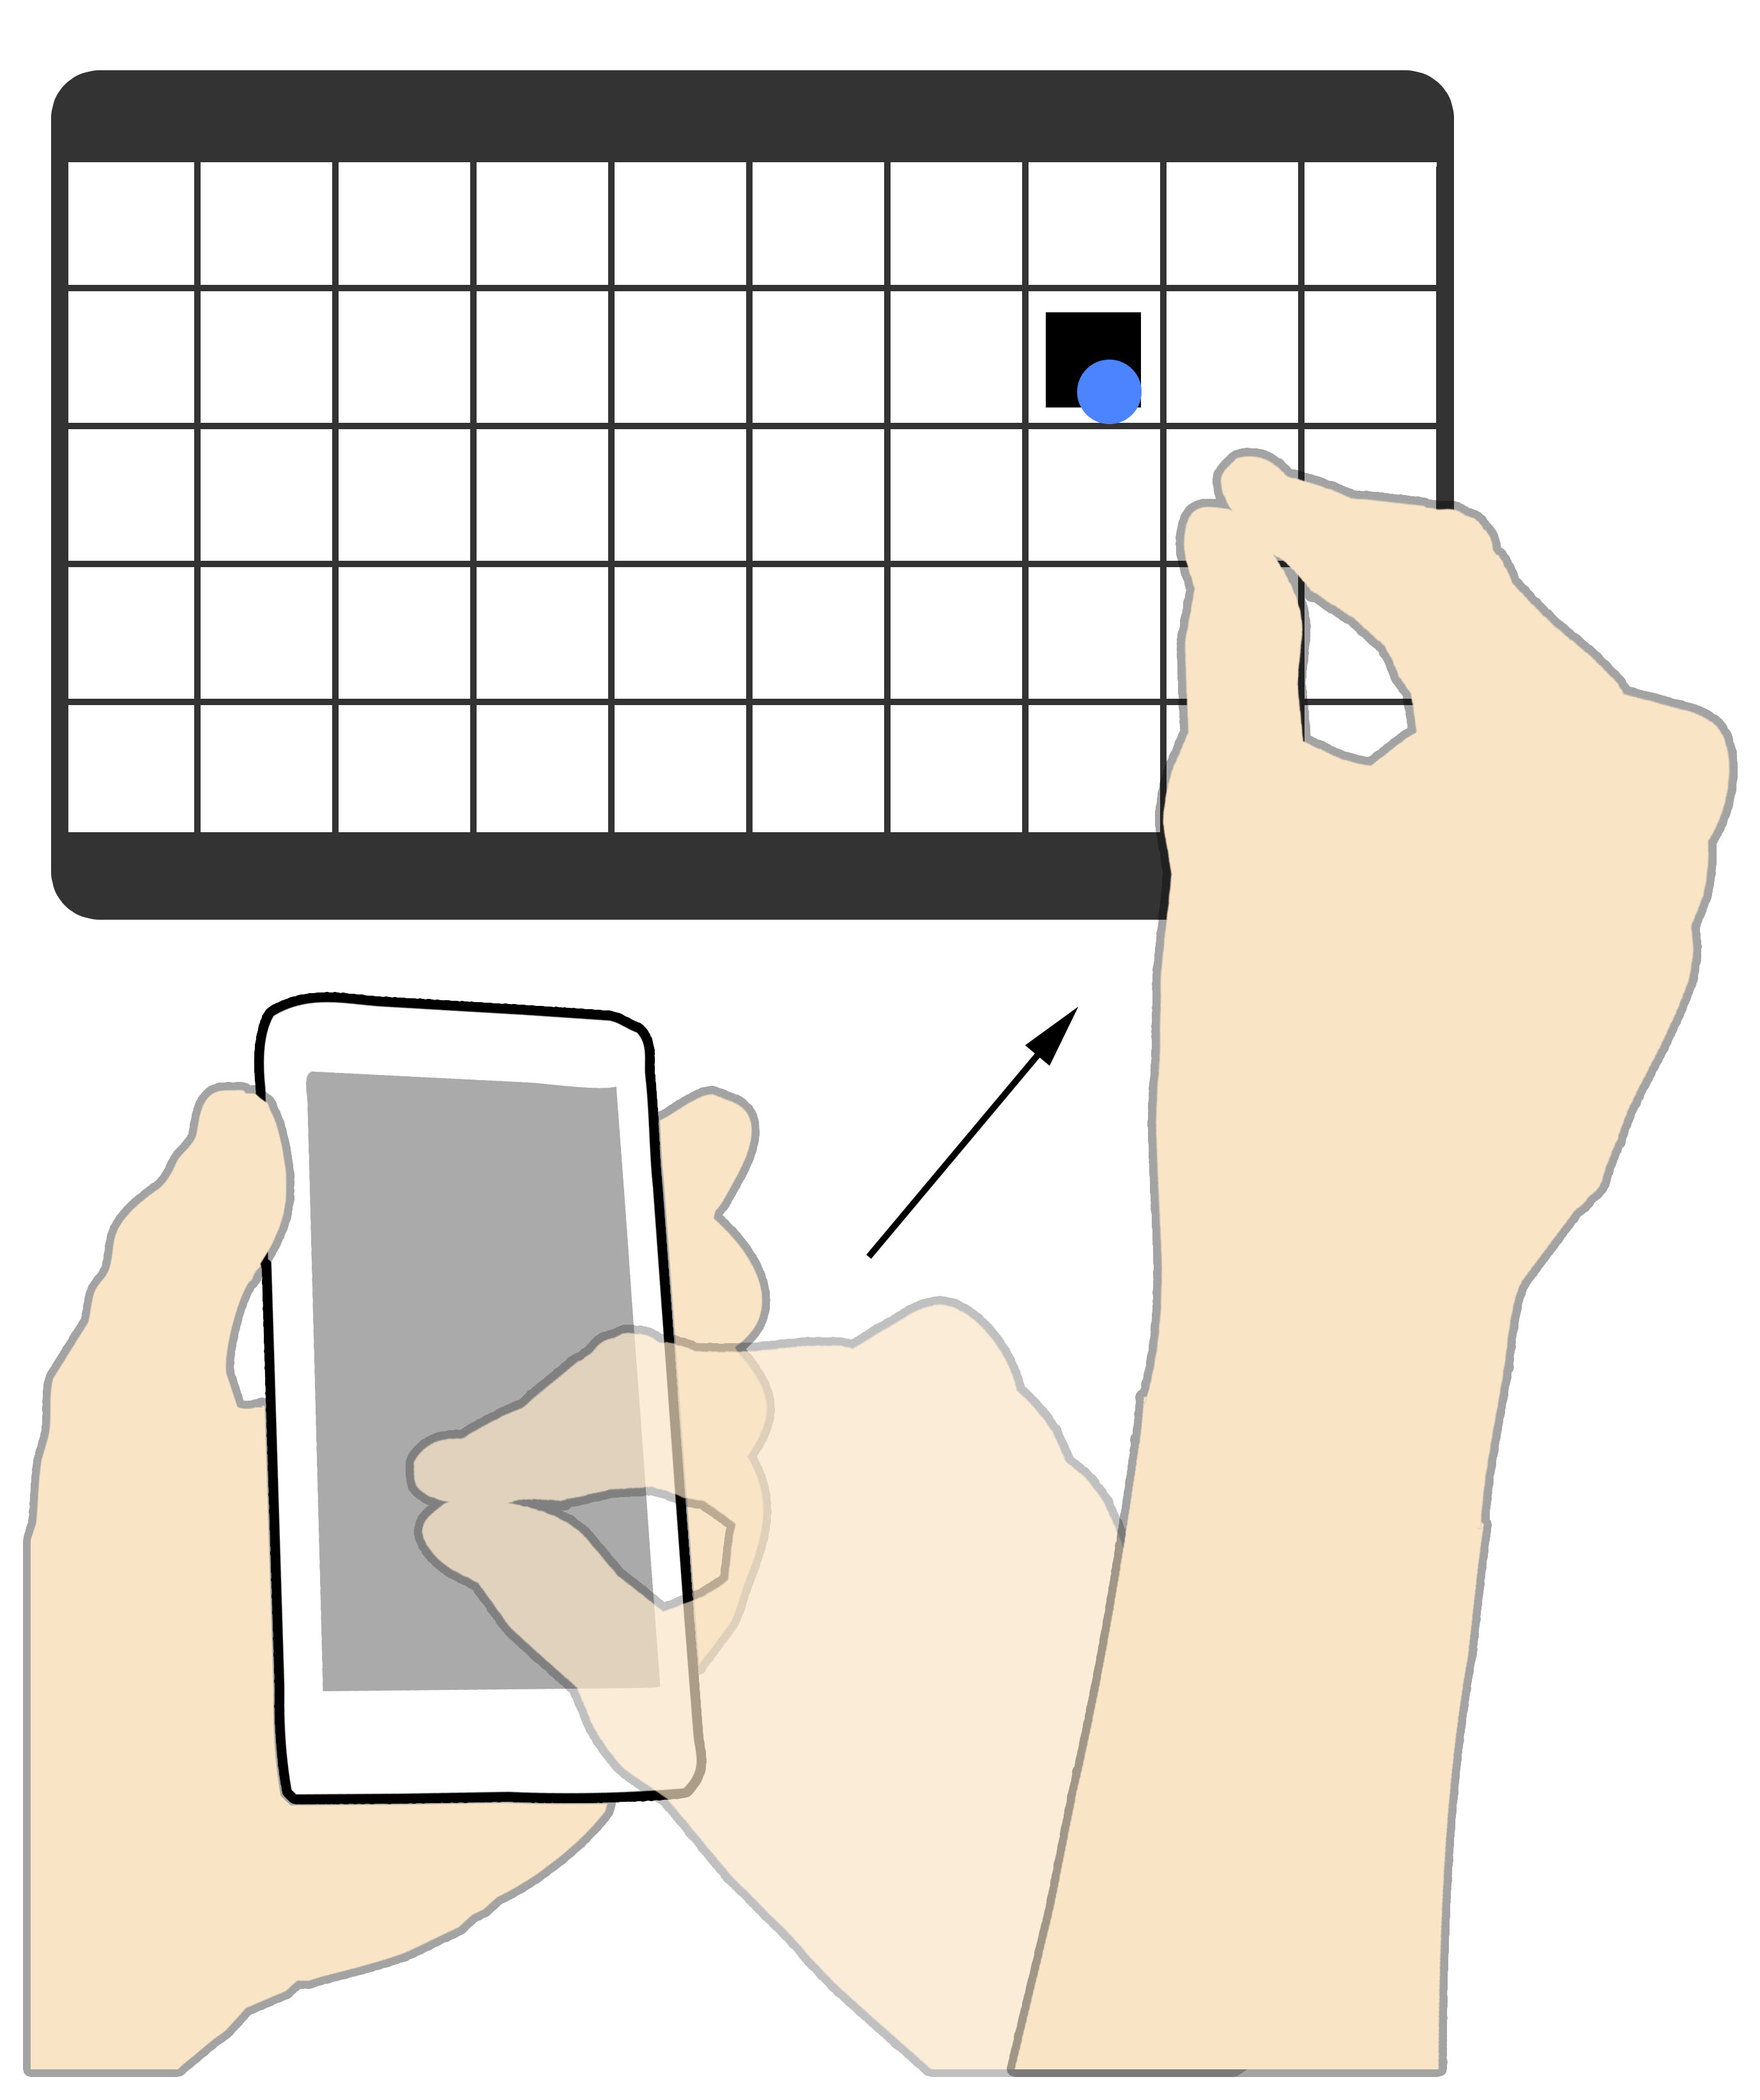
\includegraphics[width = 0.33\columnwidth]{images/techniques/grabPush2.jpg}\label{fig:grabTechniqueB}}
	\subfloat[]{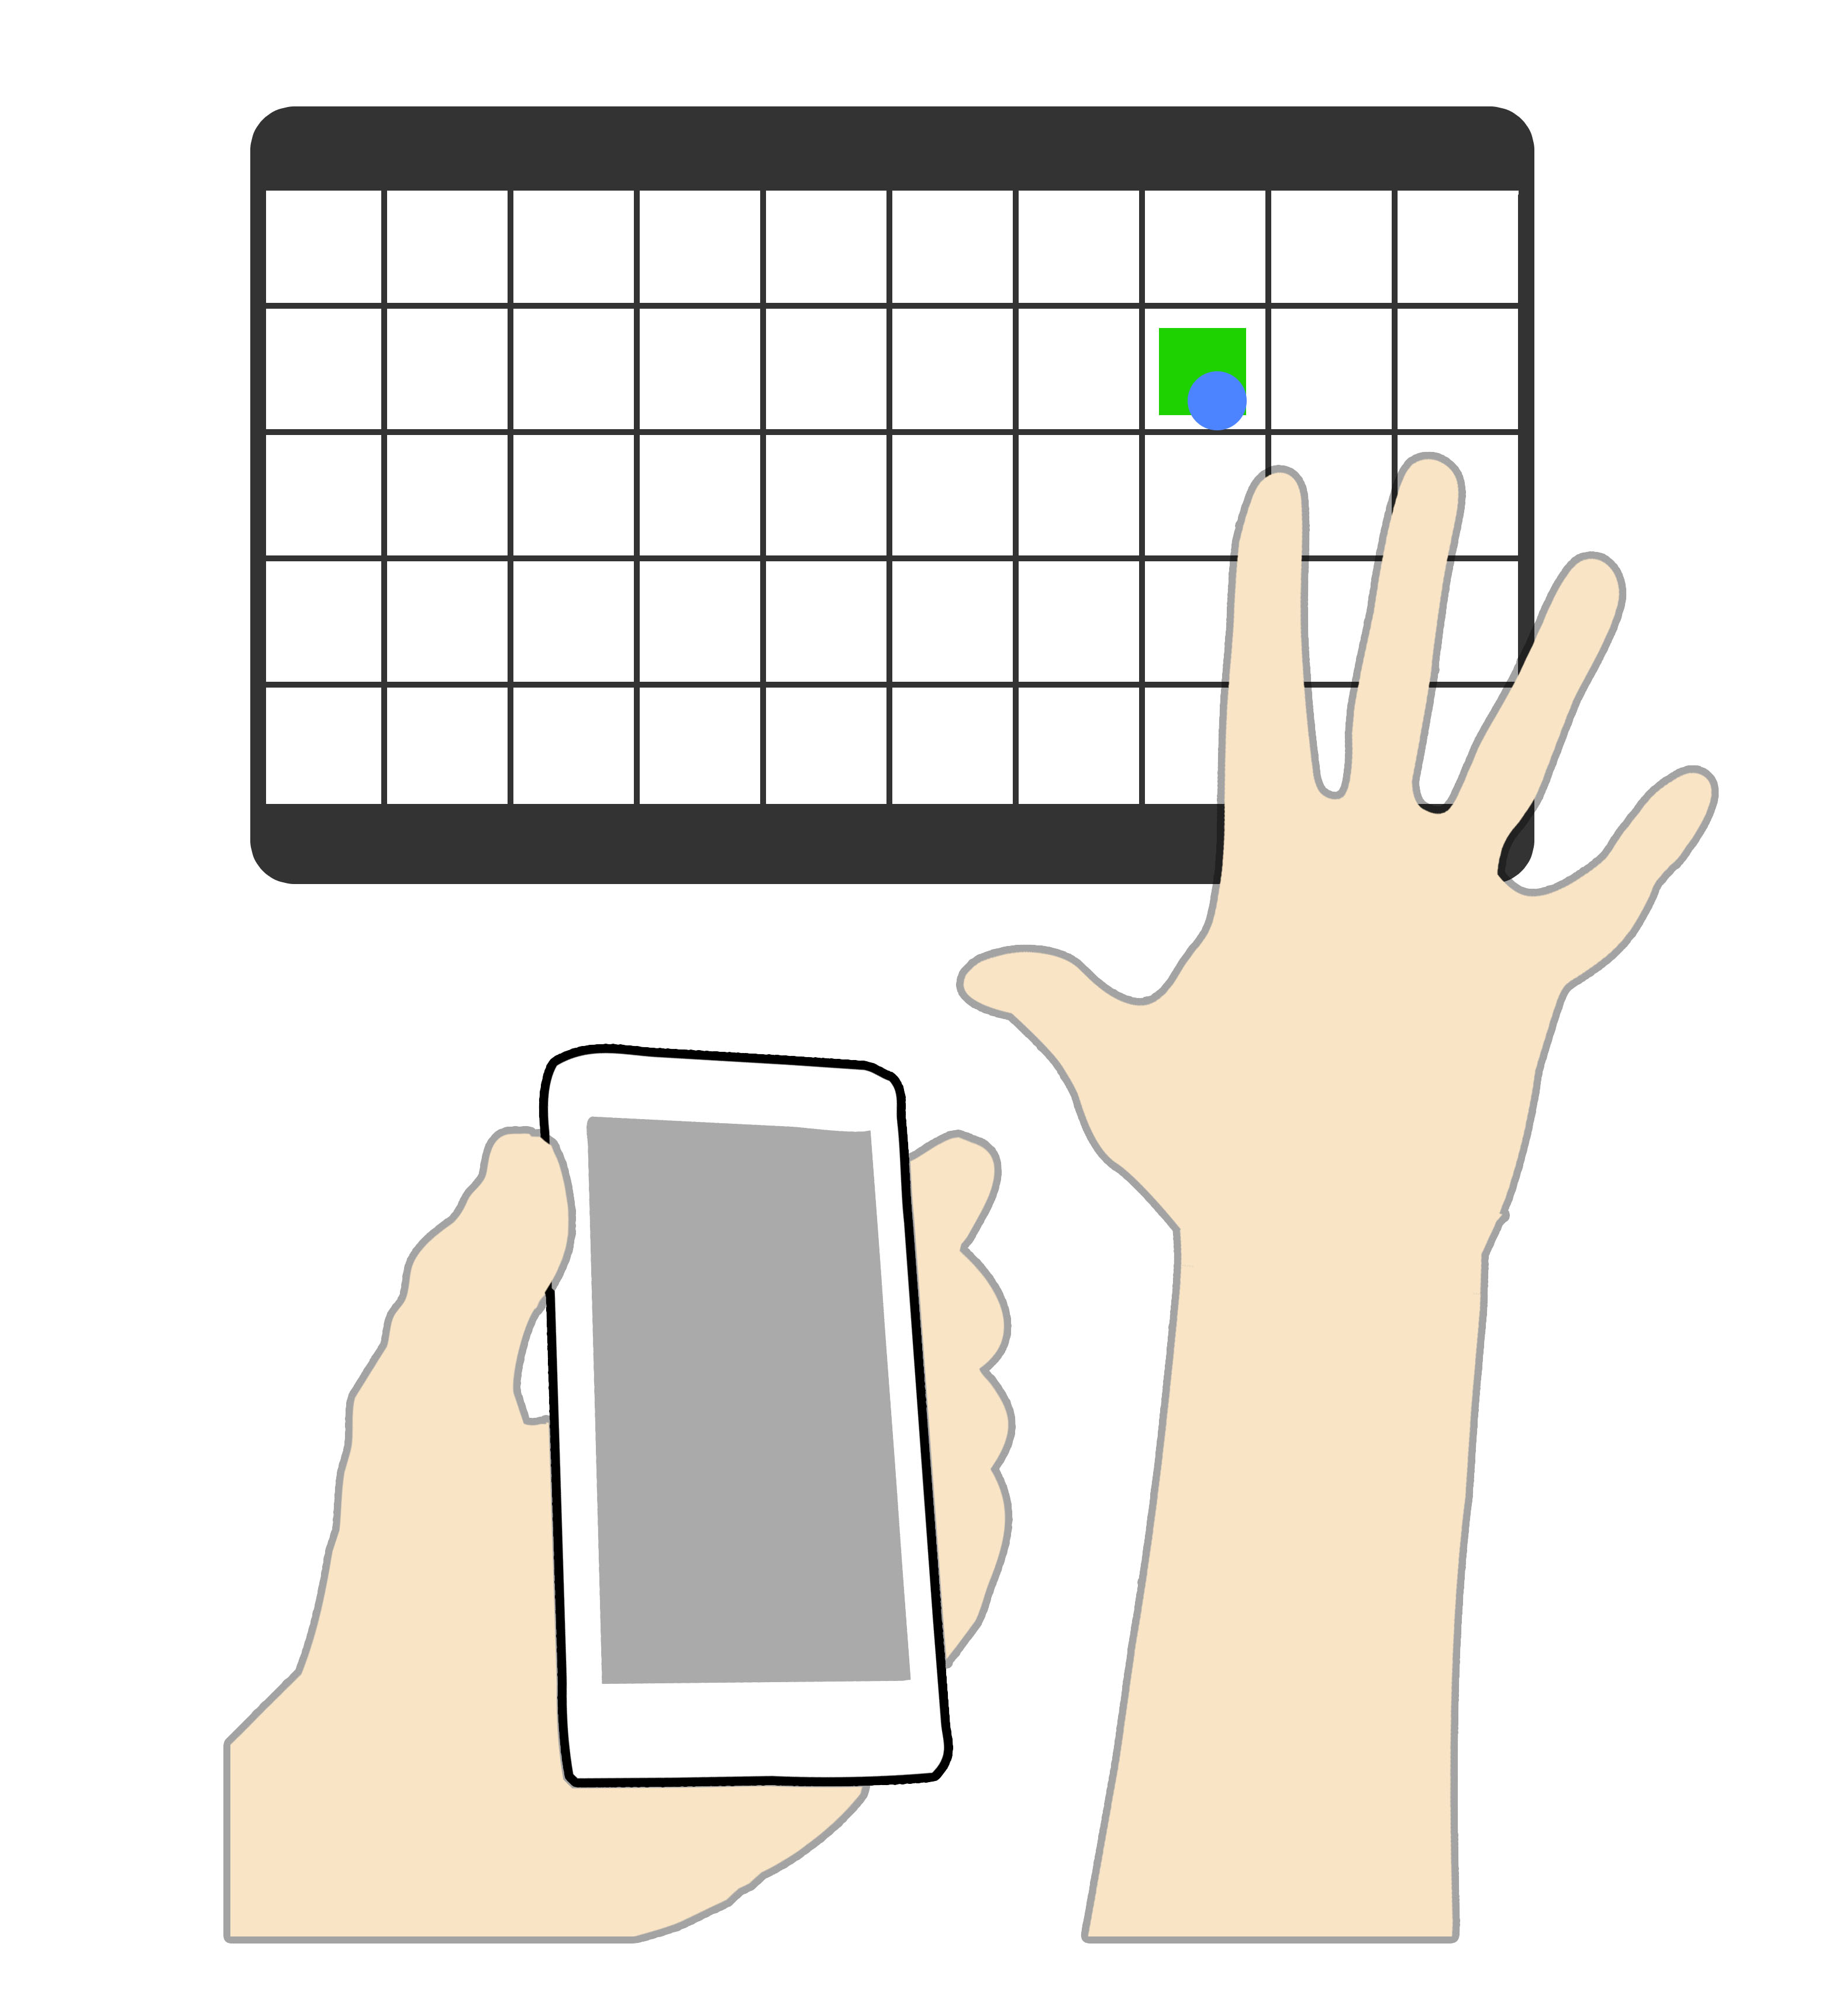
\includegraphics[width = 0.33\columnwidth]{images/techniques/grabPush3.jpg}\label{fig:grabTechniqueC}}
	\caption{\push \grab technique}
	\label{fig:grabTechnique}
\end{figure}

\subsubsection{Swipe} \label{sec:swipeTechnique}
The \swipe technique (\cref{fig:swipeTechnique}) was utilized by Bragdon et. al in \emph{Code Space} \cite{Bragdon:2011}.
They developed a system that would support developer meetings with the help of smart phones and the Kinect. 
Bragdon et al. describe the technique as \emph{``cross-device interaction with touch and air pointing''} and the swiping motion is described as \emph{``flicking up on the touch screen''}.
This technique was chosen because it has a very simplistic design, with a very low level of complexity since it requires very few steps to activate.
It is also a one handed technique and requires very little effort from the user to use.
The \push and \pull version of this technique are very similar.
First the user points at the desired location with the phone using a stretched arm (\cref{fig:swipeTechniqueA}) and then swipes his finger on the screen (\cref{fig:swipeTechniqueC}).
The direction he swipes depends on whether the user wants to \push or \pull information.
If he swipes away from himself, he pushes information to the screen.
If he swipes towards himself, he is pulling information from the screen onto the device.  

\begin{figure}[H]
	\subfloat[]{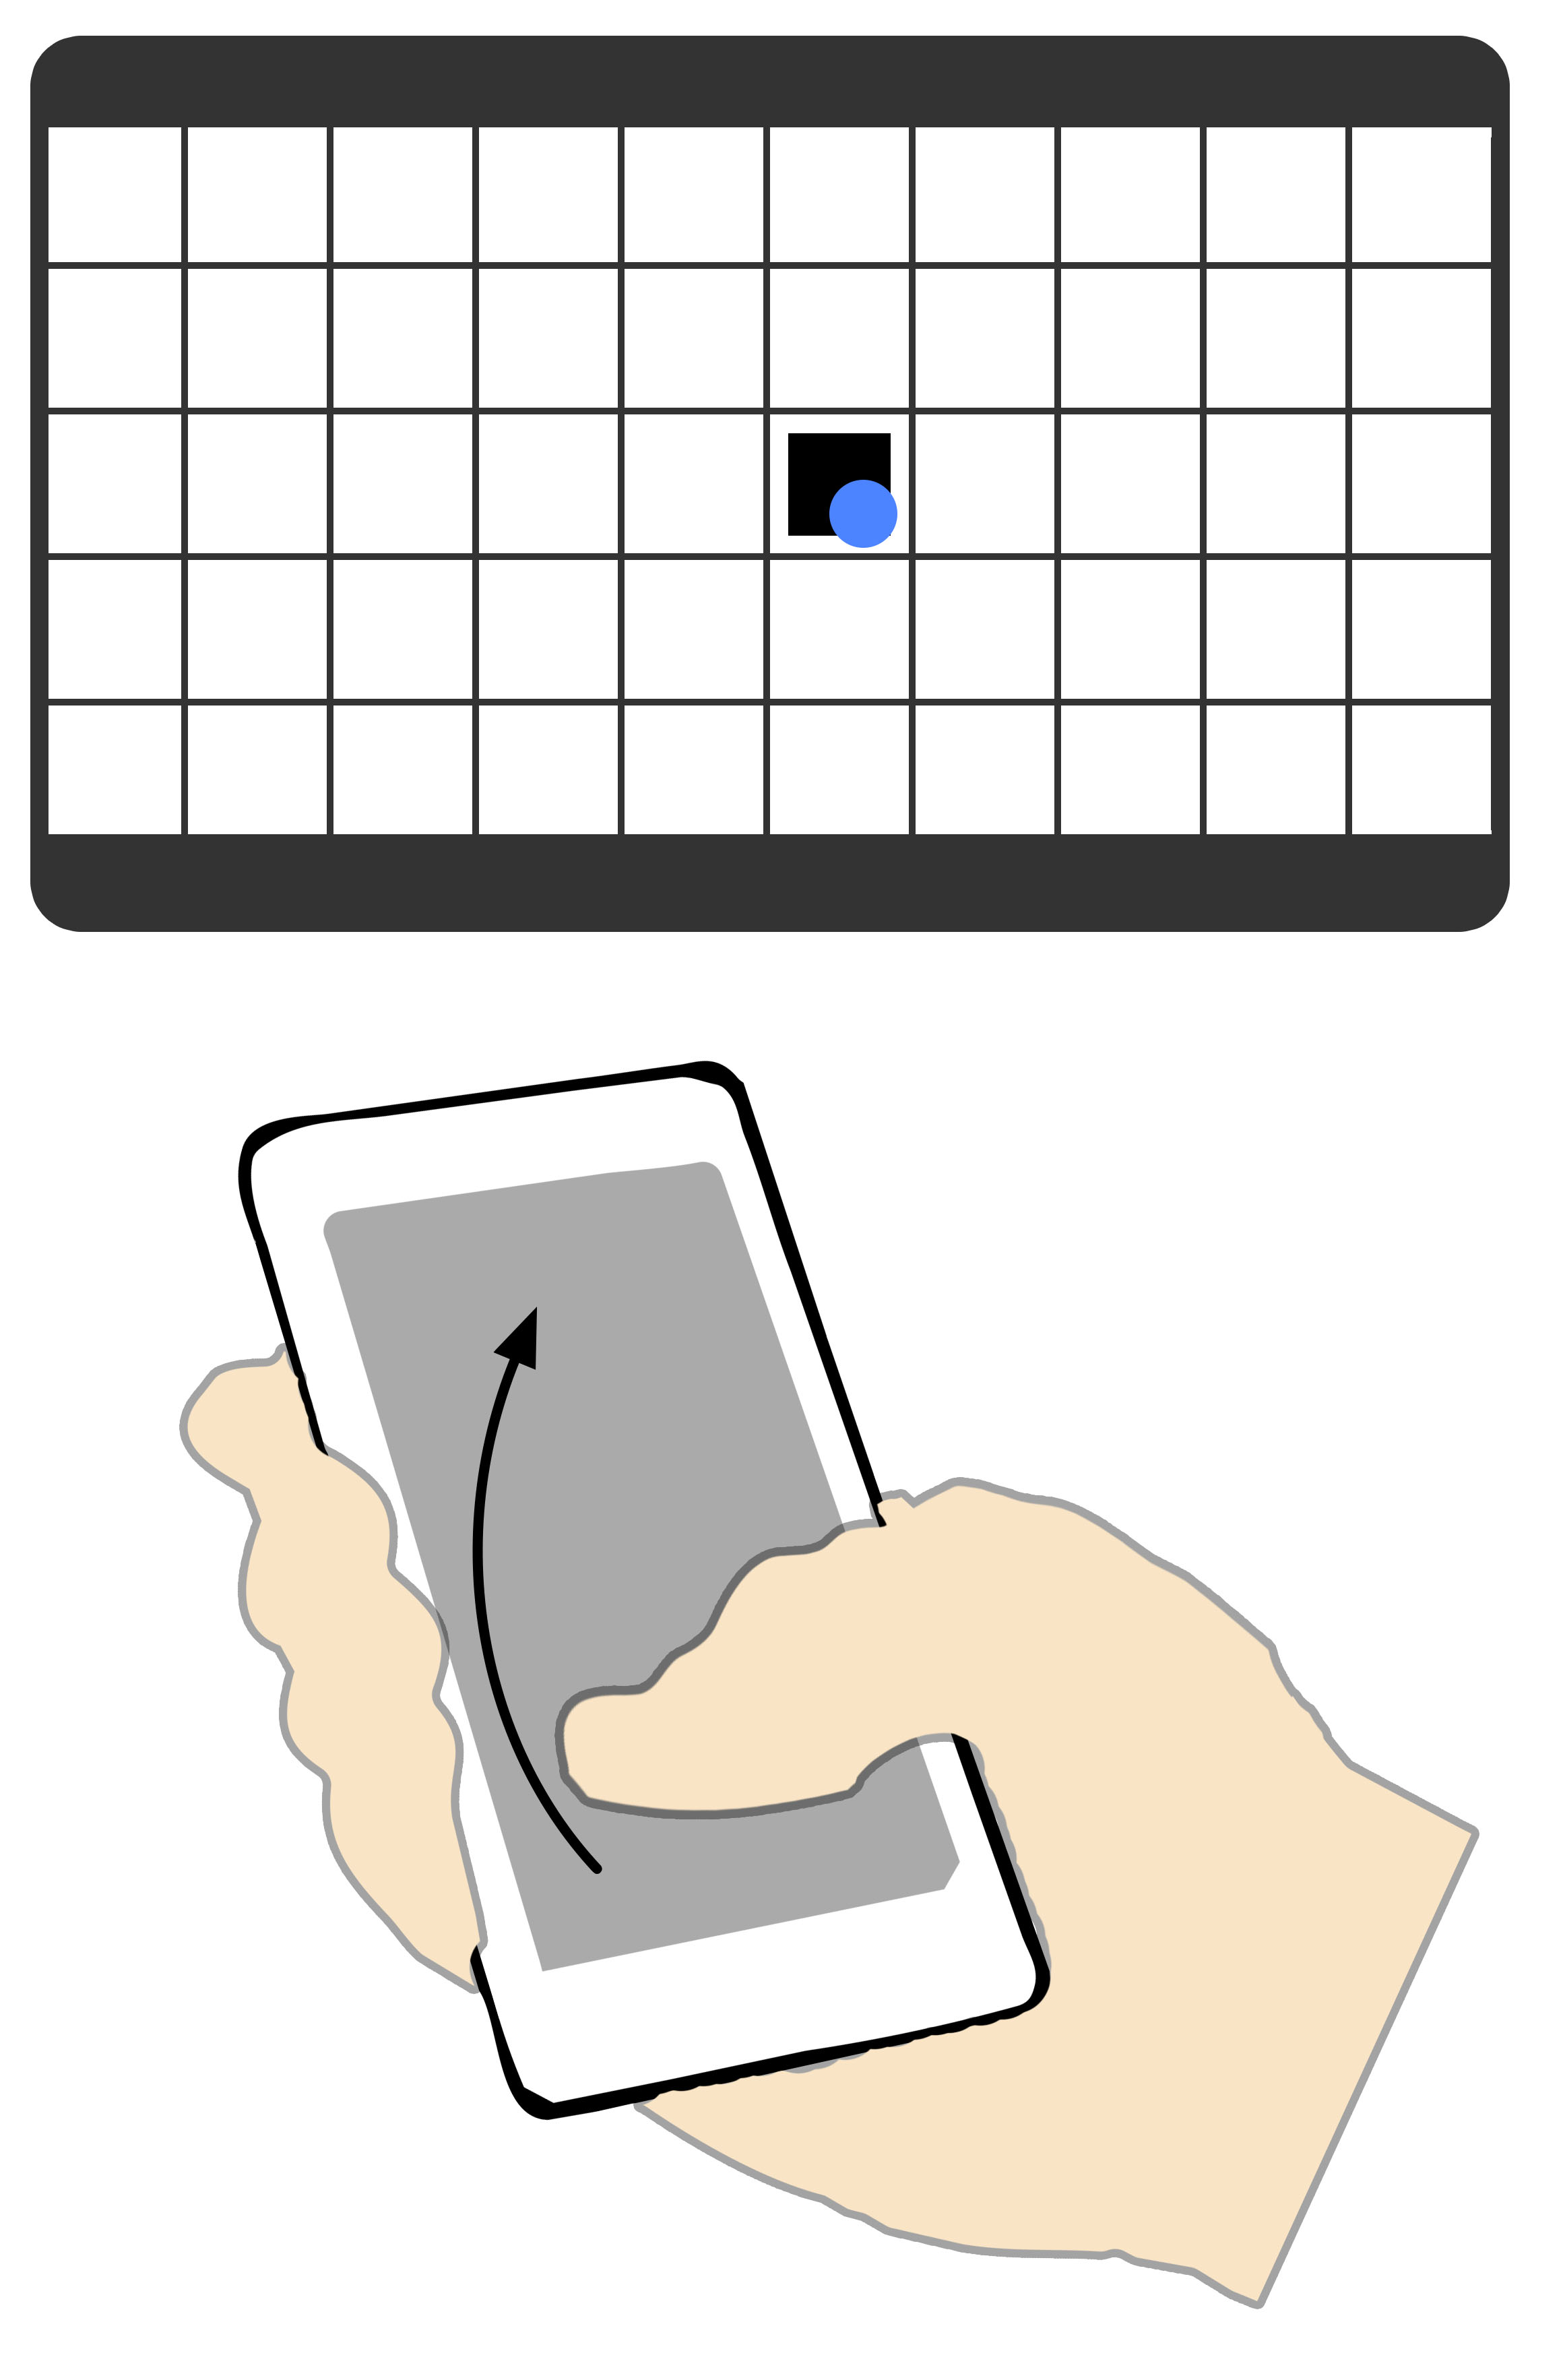
\includegraphics[width = 0.33\columnwidth]{images/techniques/swipePush1.jpg}\label{fig:swipeTechniqueA}}
	\subfloat[]{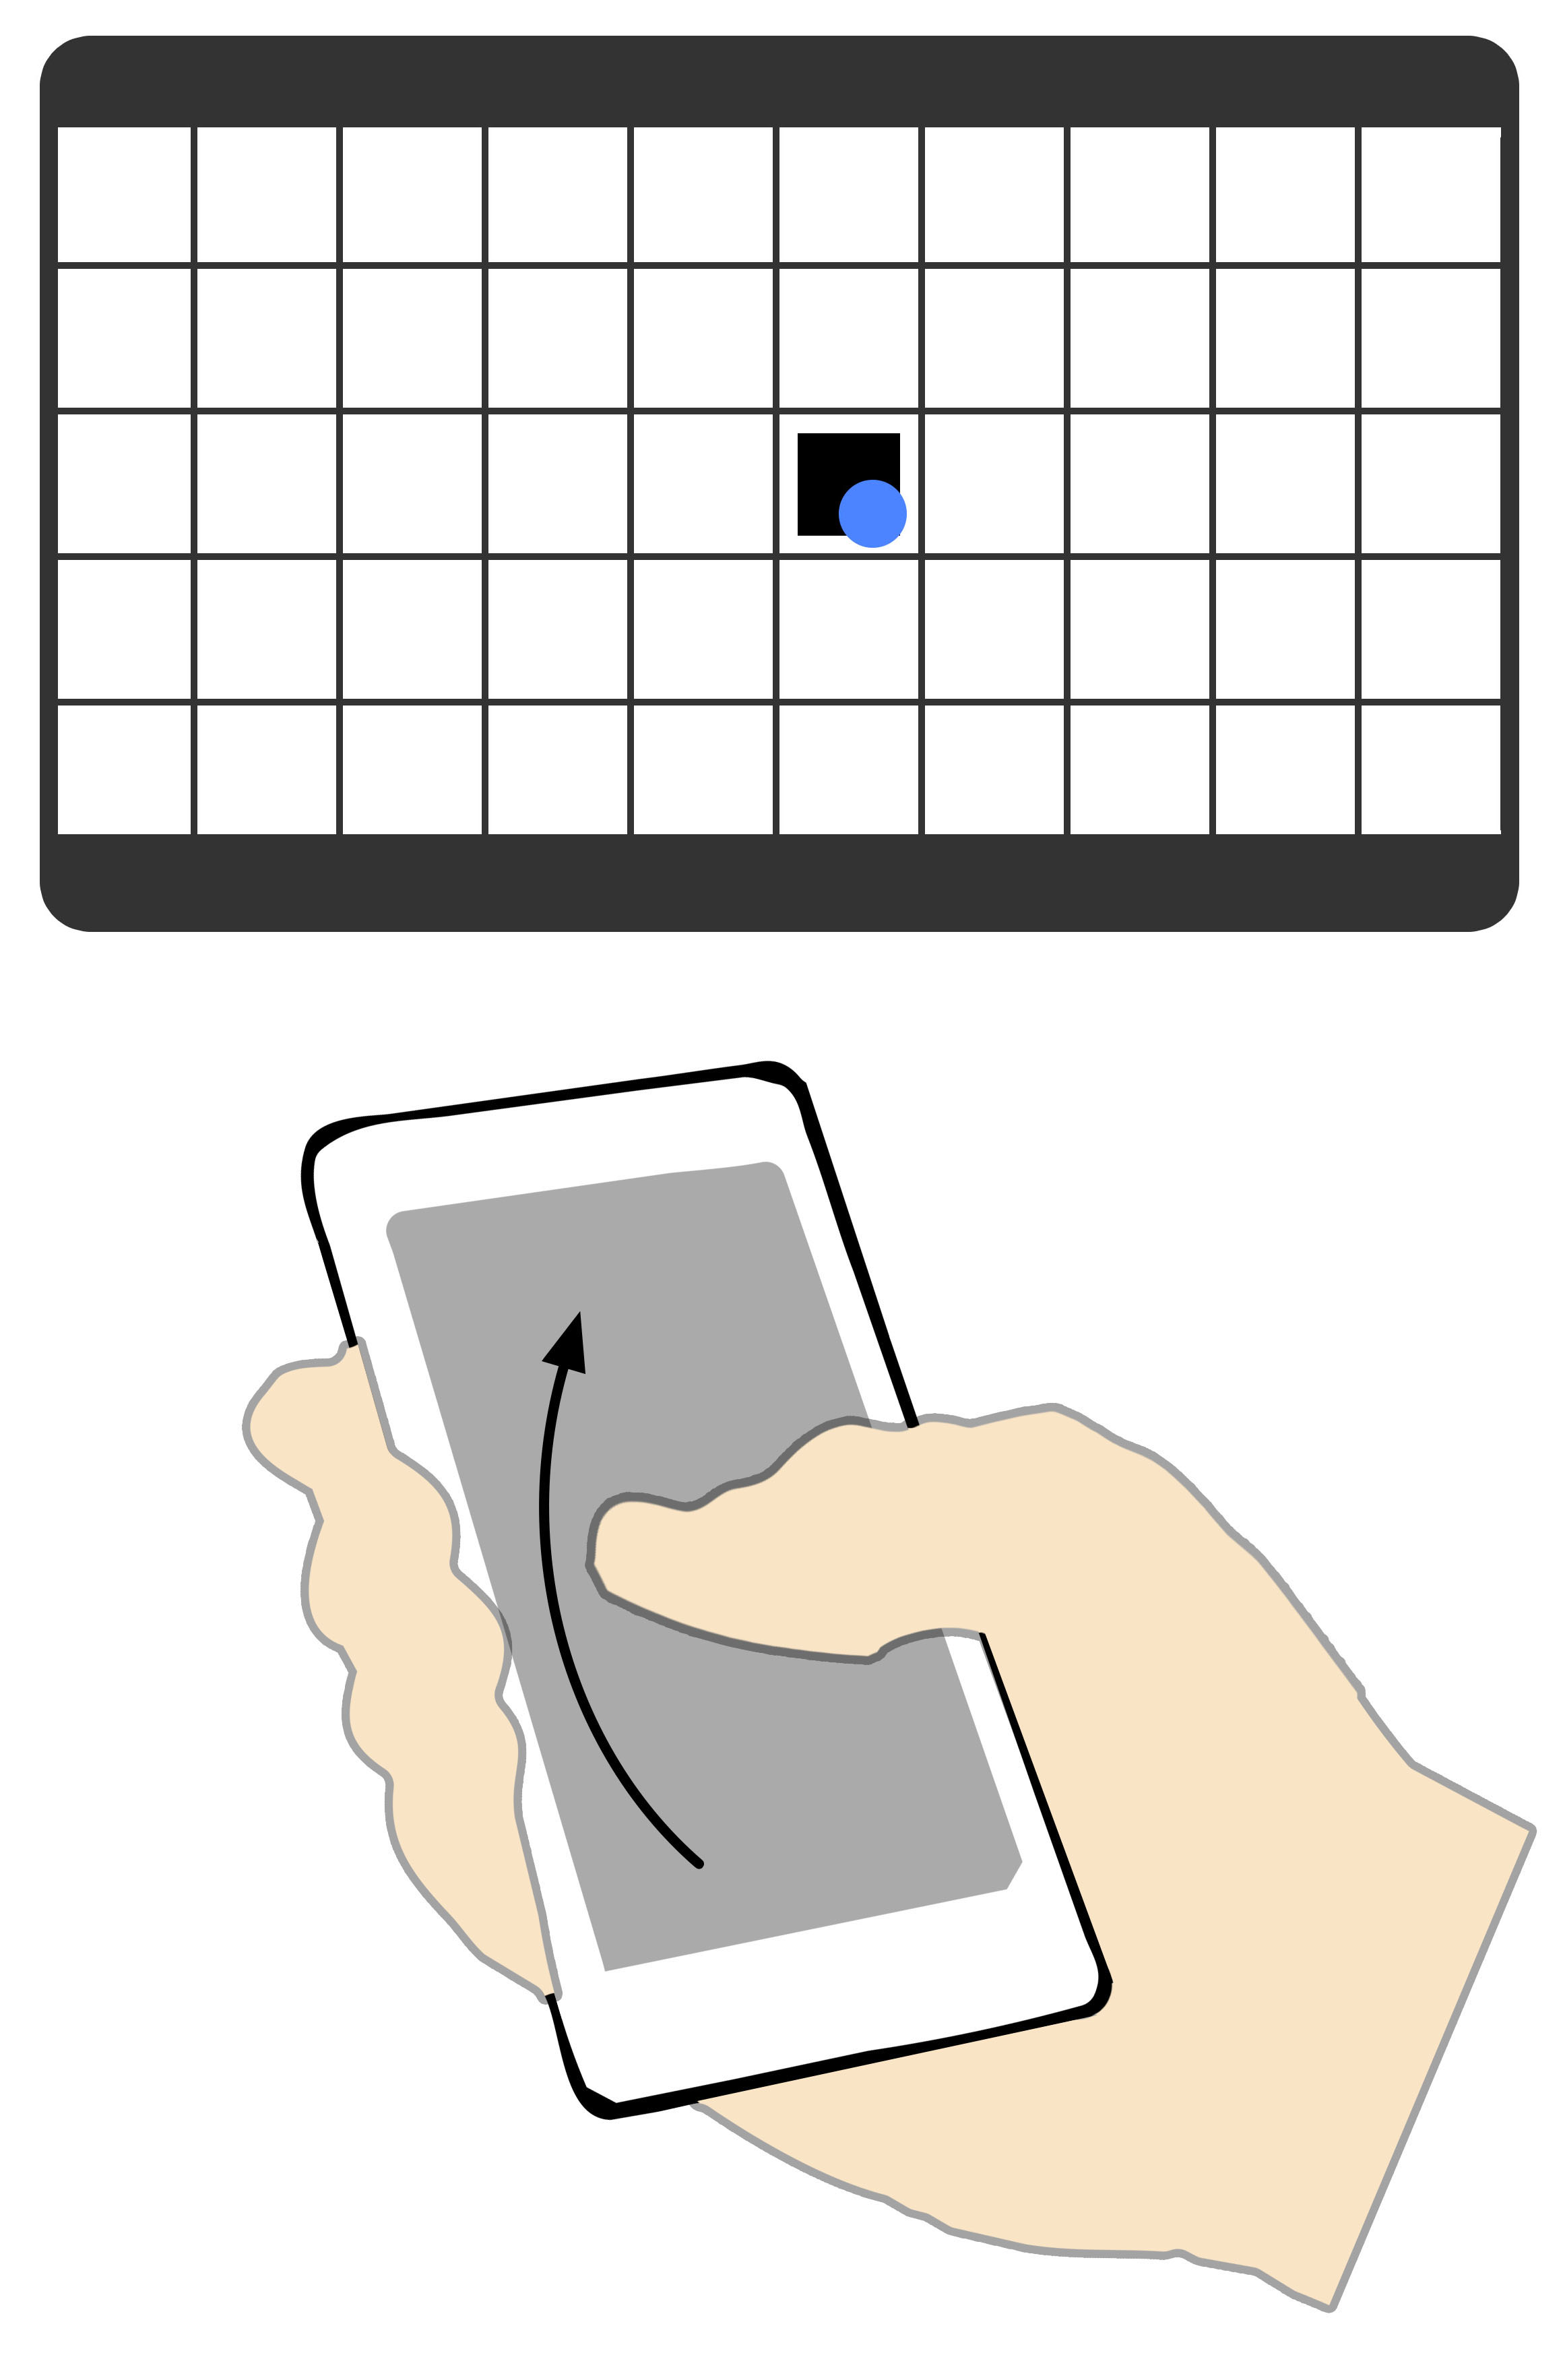
\includegraphics[width = 0.33\columnwidth]{images/techniques/swipePush2.jpg}\label{fig:swipeTechniqueB}}
	\subfloat[]{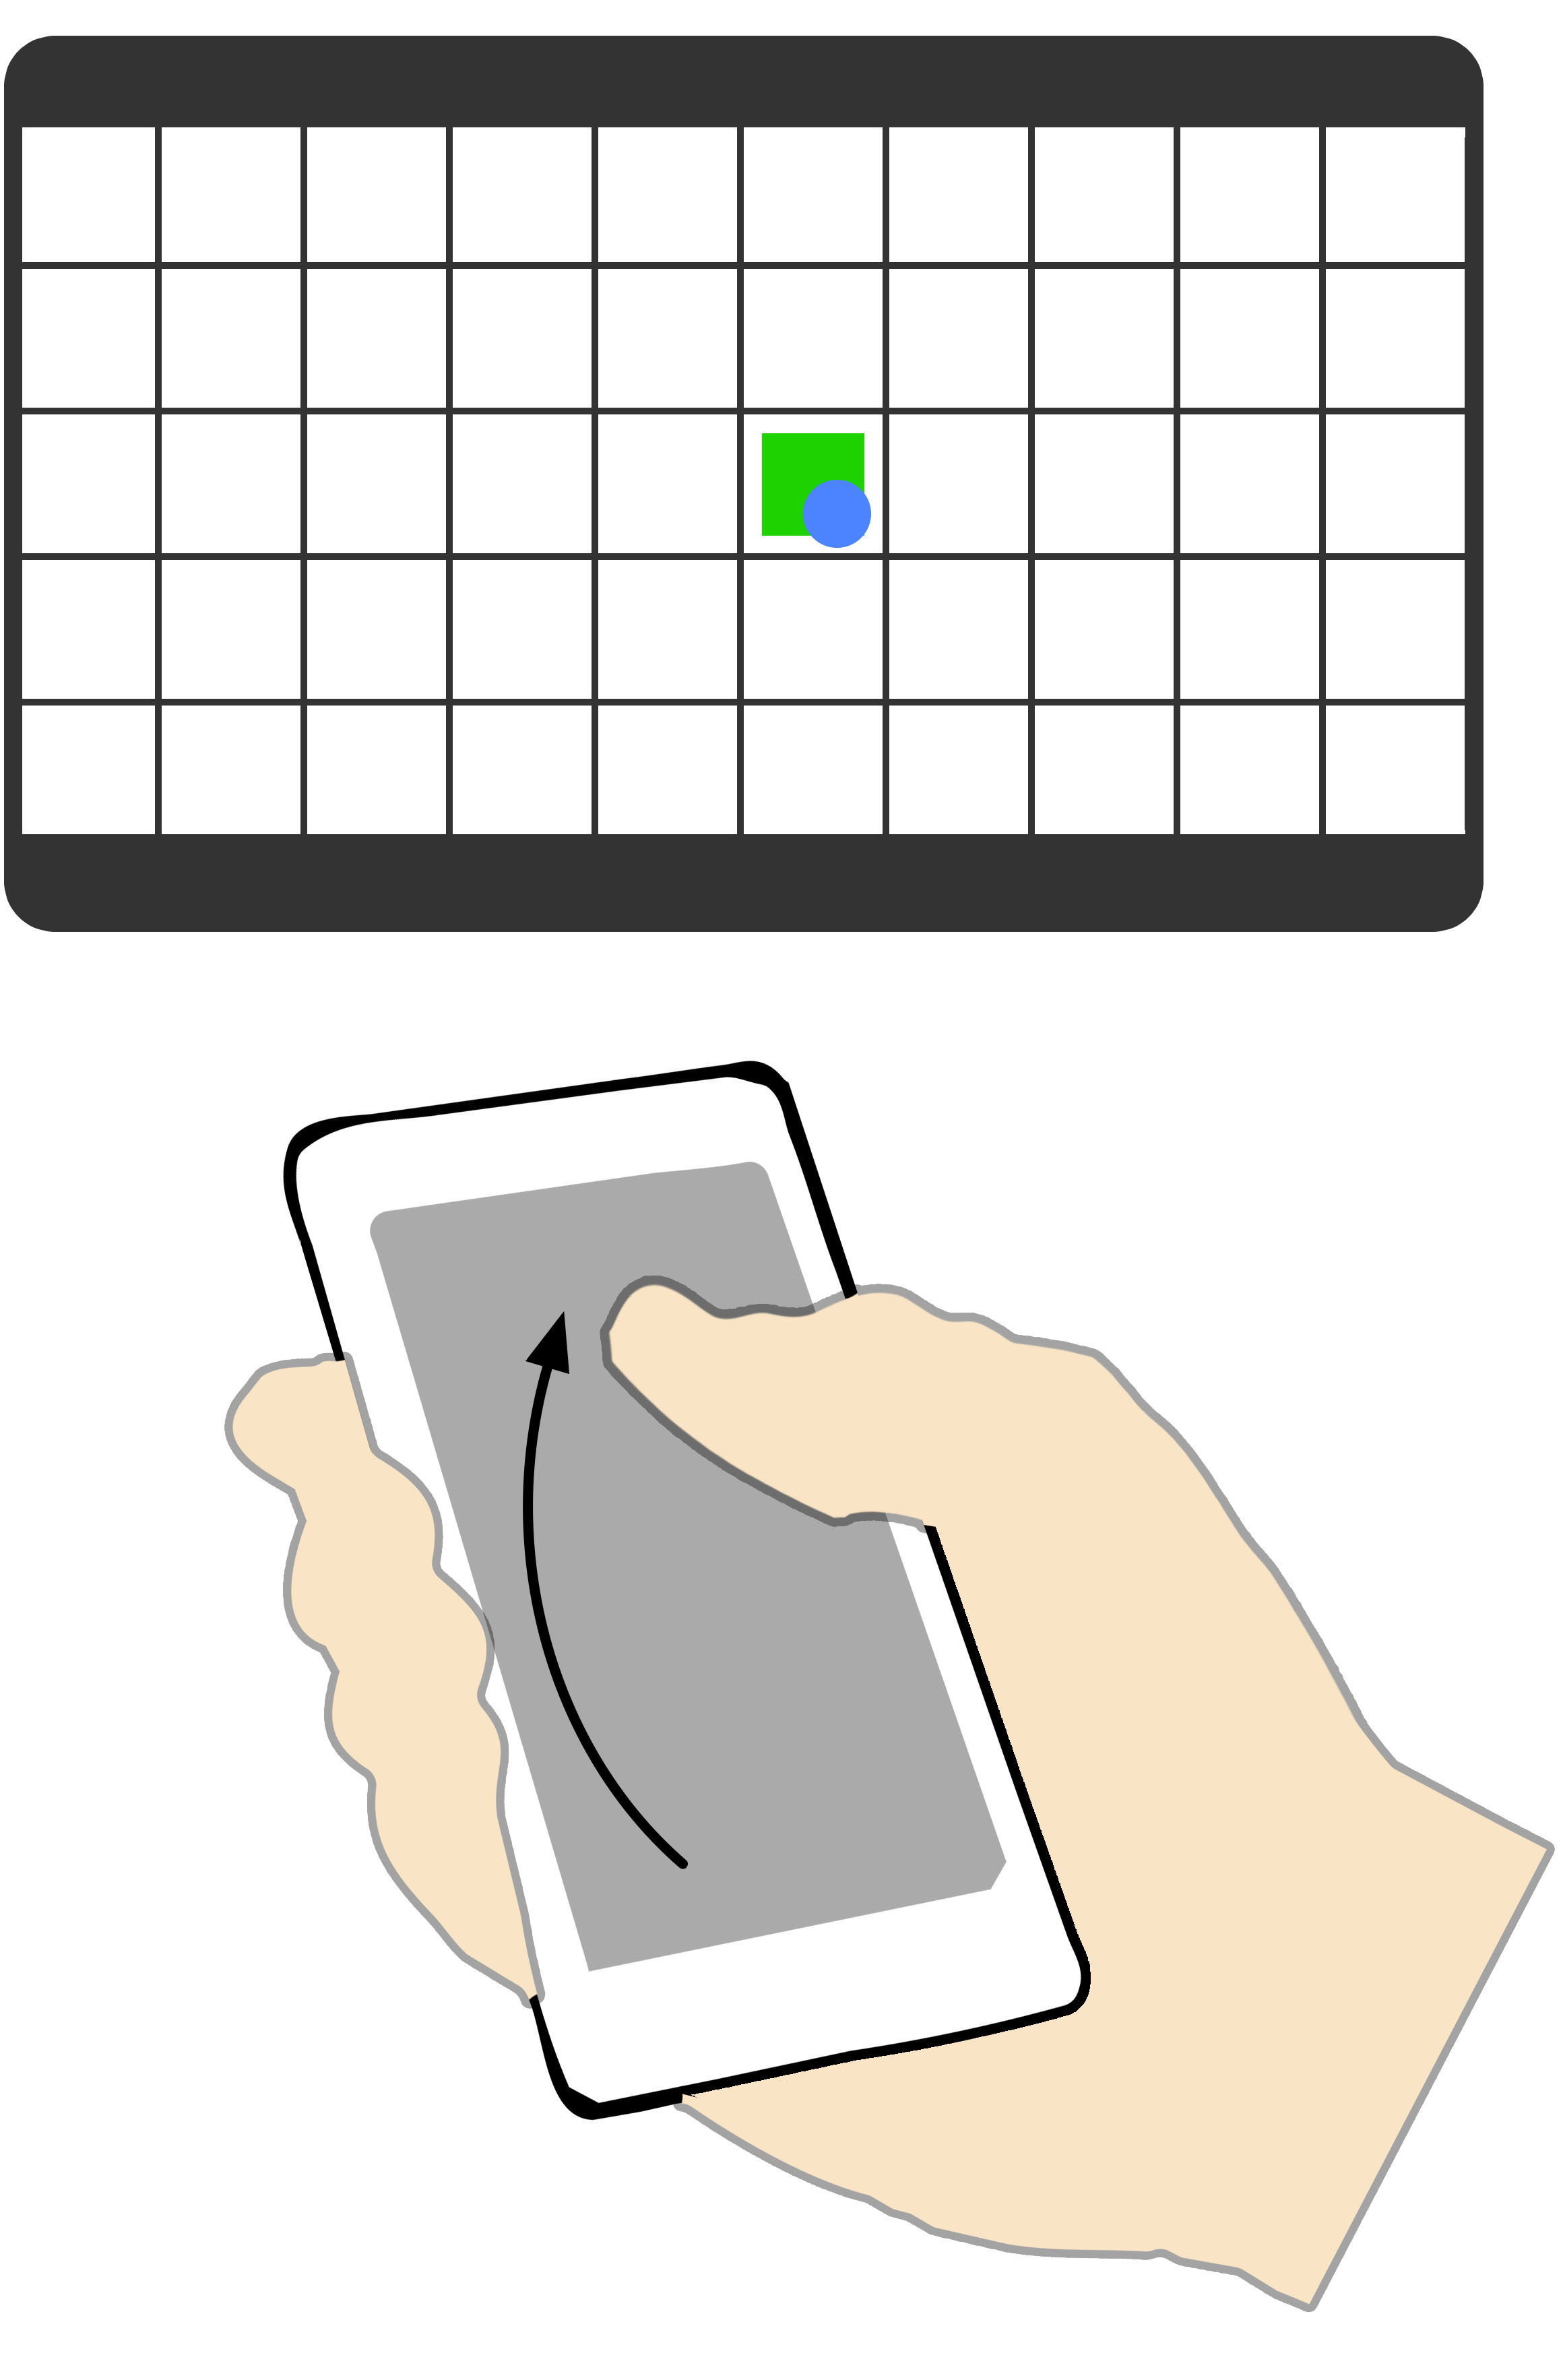
\includegraphics[width = 0.33\columnwidth]{images/techniques/swipePush3.jpg}\label{fig:swipeTechniqueC}}
	\caption{\push \swipe technique}
	\label{fig:swipeTechnique}
\end{figure}

\subsubsection{Throw} \label{sec:throwTechnique}
The \throw technique (\cref{fig:throwTechnique}) is a combination of two techniques.
The first is a pointing technique used by Walter et al. in \emph{Cuenesics} \cite{Walter:2014} were the user uses his hands to control a cursor on the screen.
The second is a technique used by Yatani et al. \cite{Yatani:2005} in \emph{Toss-it} to throw information between handheld devices and by Scheible et al. in \emph{MobiToss} \cite{Scheible:2008} were the system is used to submit information onto a large public display.
This technique was chosen because of its natural and playful design, as well as mirroring the idea of throwing something, like a ball, somewhere or to someone.
\throw is a two handed technique, as well as having a larger number of steps to take in order to activate it.
The \throw technique is performed as follows: 
First the user points at the targeted position with a finger (\cref{fig:throwTechniqueA}).
Then, if the user is pushing data from the phone, he has to select the data to be pushed (\cref{fig:throwTechniqueB}).
The user then performs a swinging motion with the hand which is holding the phone.
If he is pushing, then he swings towards the screen(\cref{fig:throwTechniqueC}), if he is pulling he swings away from it. 


\begin{figure}[H]
	\subfloat[]{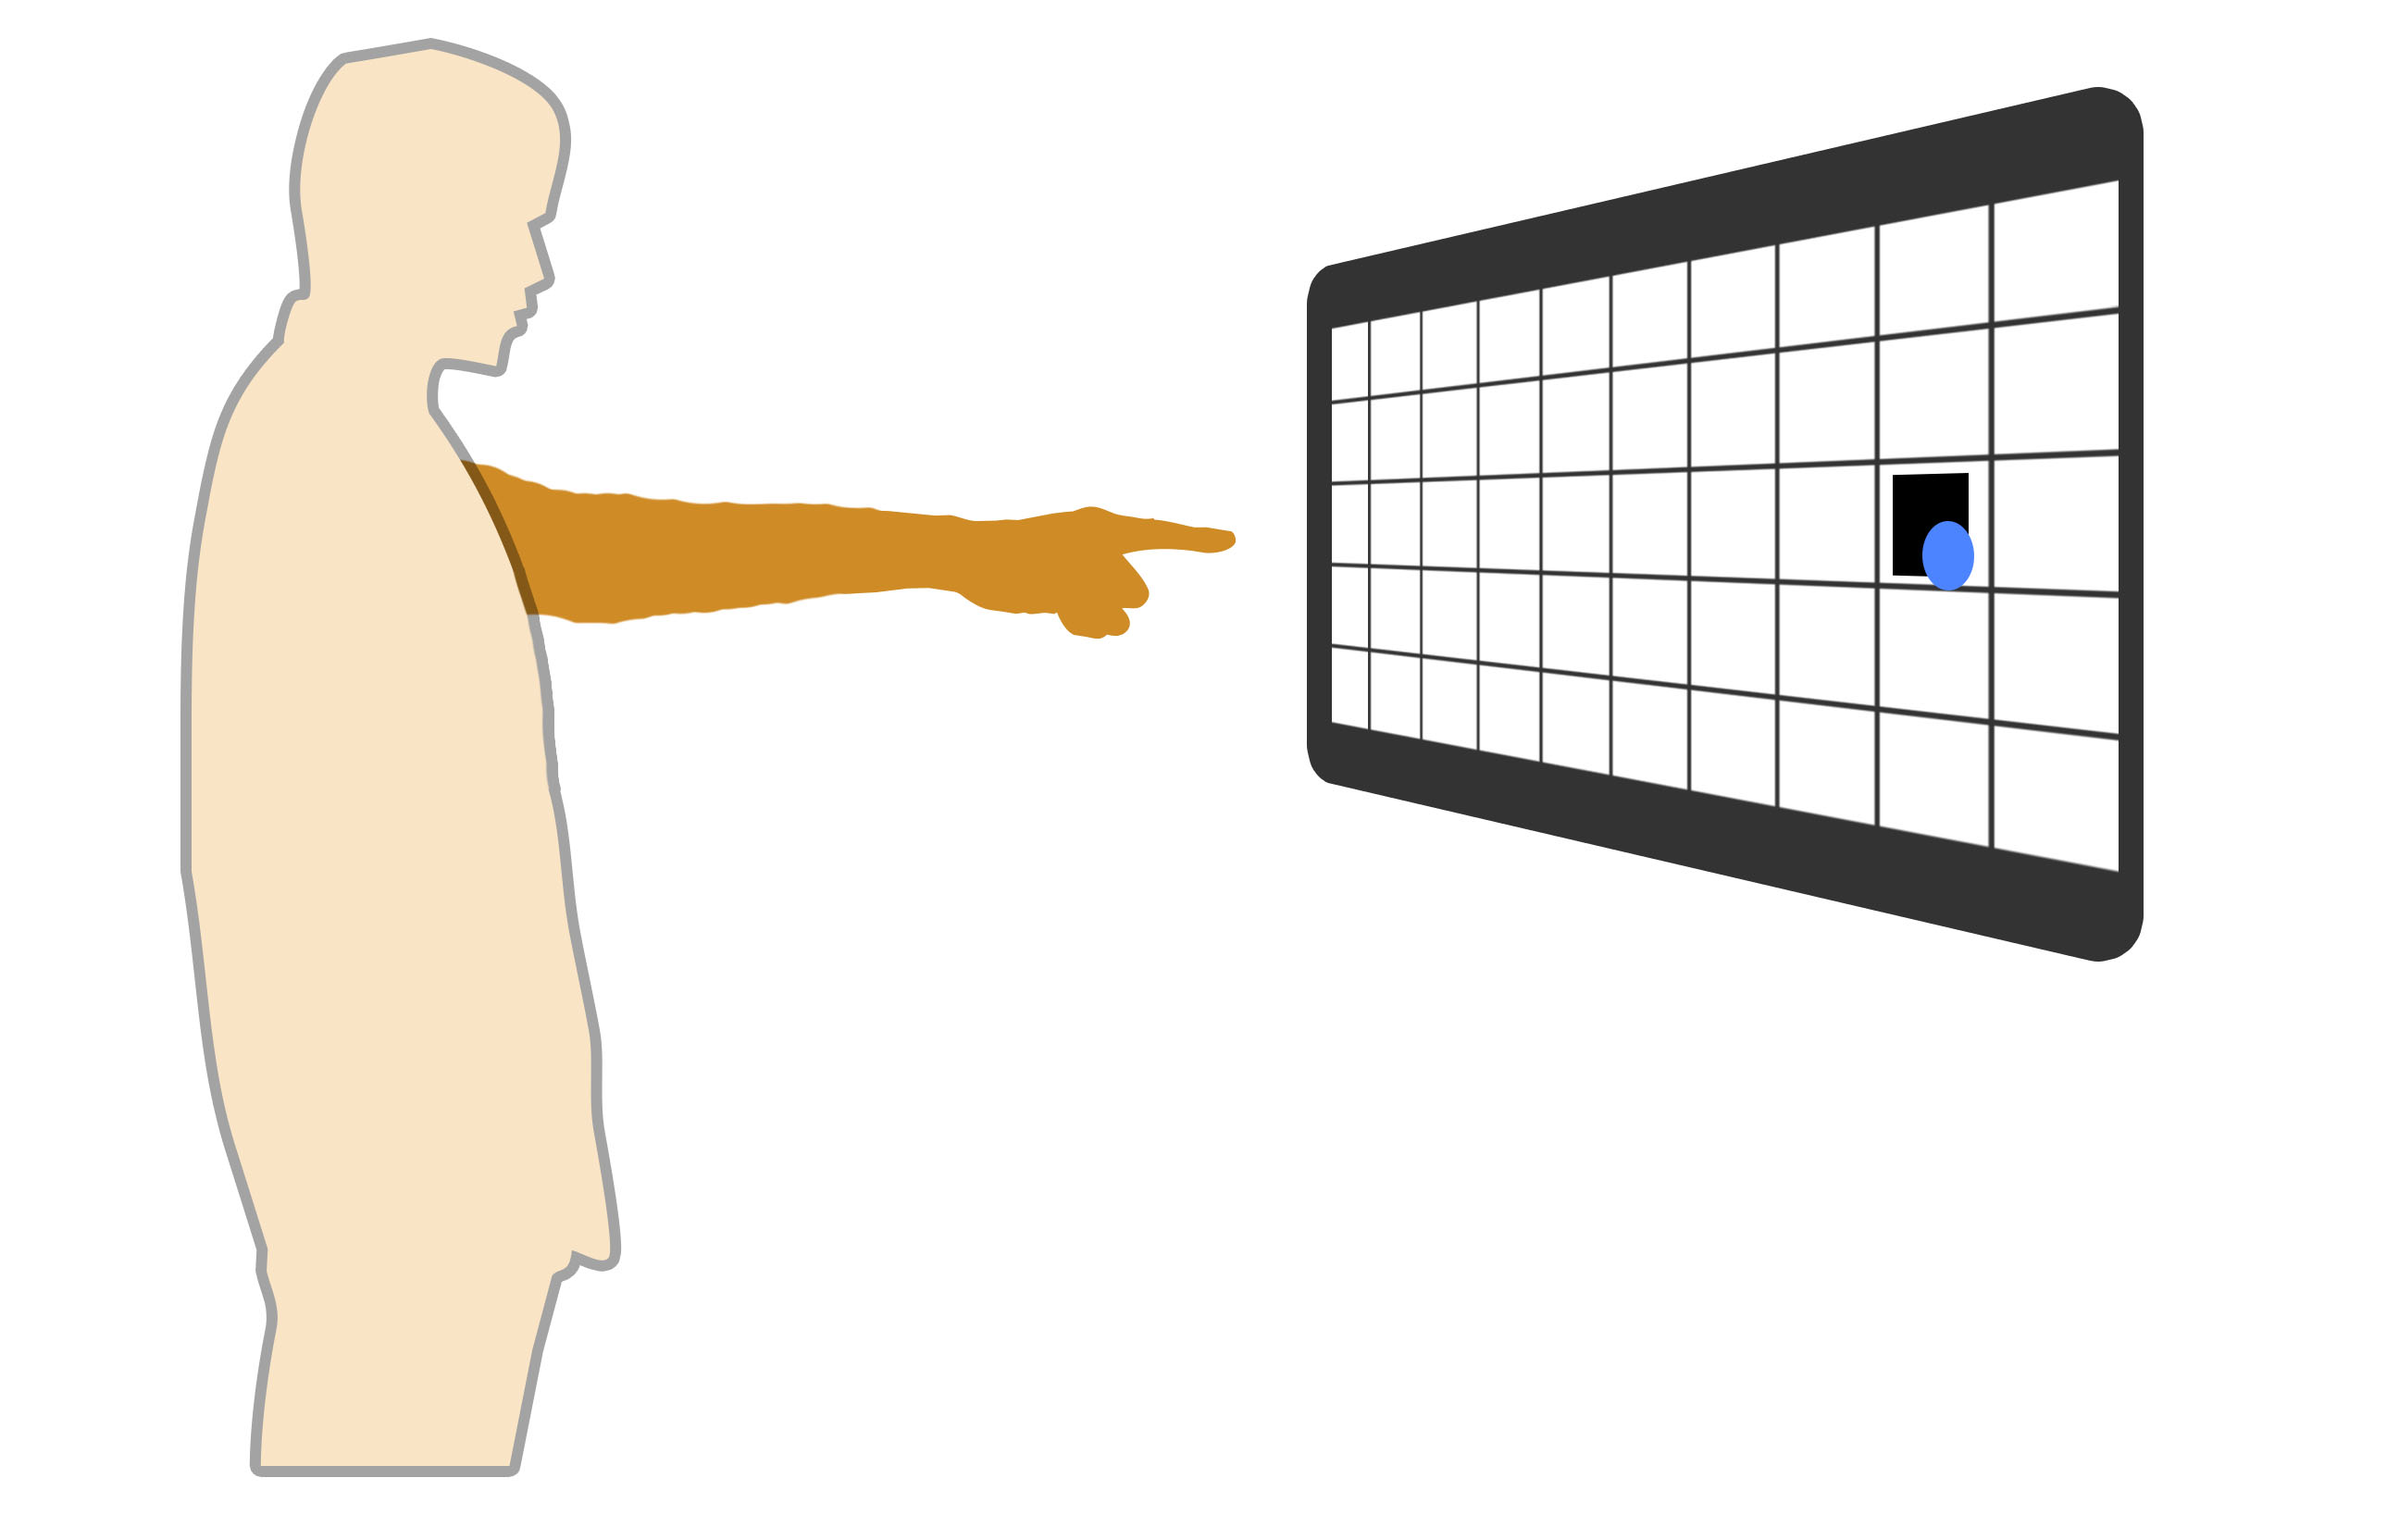
\includegraphics[width = 0.33\columnwidth]{images/techniques/throwPush1.jpg}\label{fig:throwTechniqueA}}
	\subfloat[]{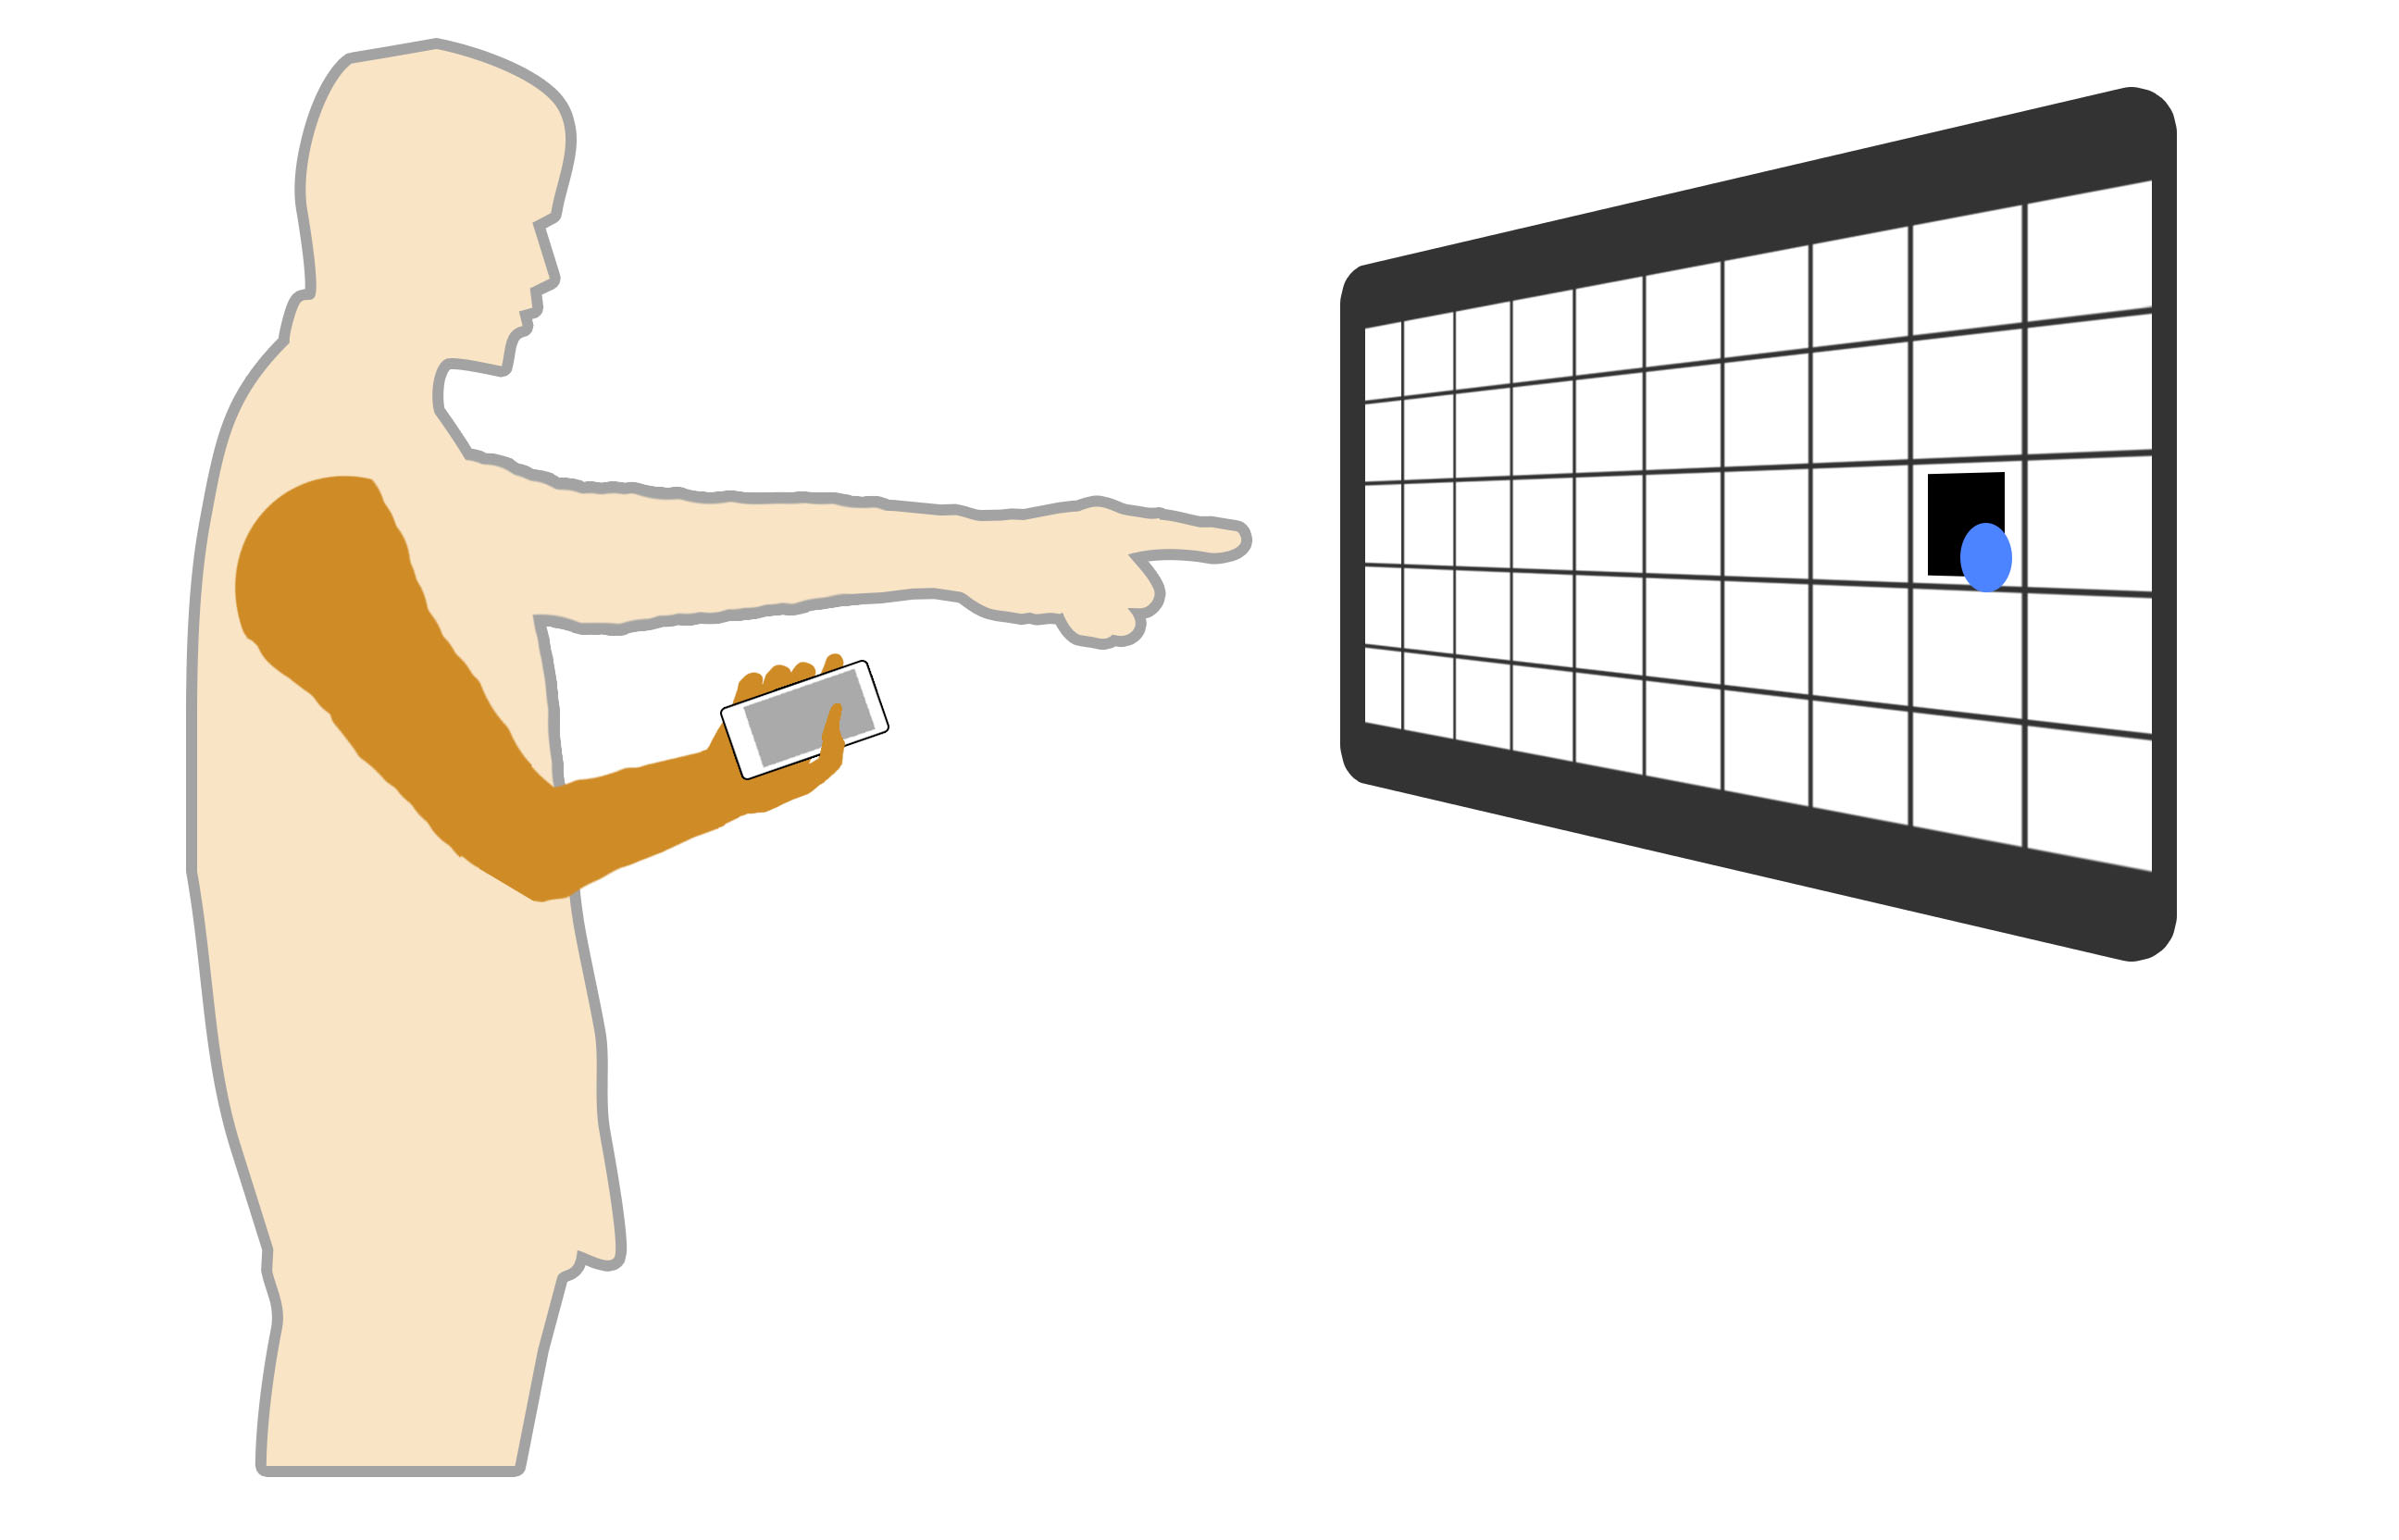
\includegraphics[width = 0.33\columnwidth]{images/techniques/throwPush2.jpg}\label{fig:throwTechniqueB}}
	\subfloat[]{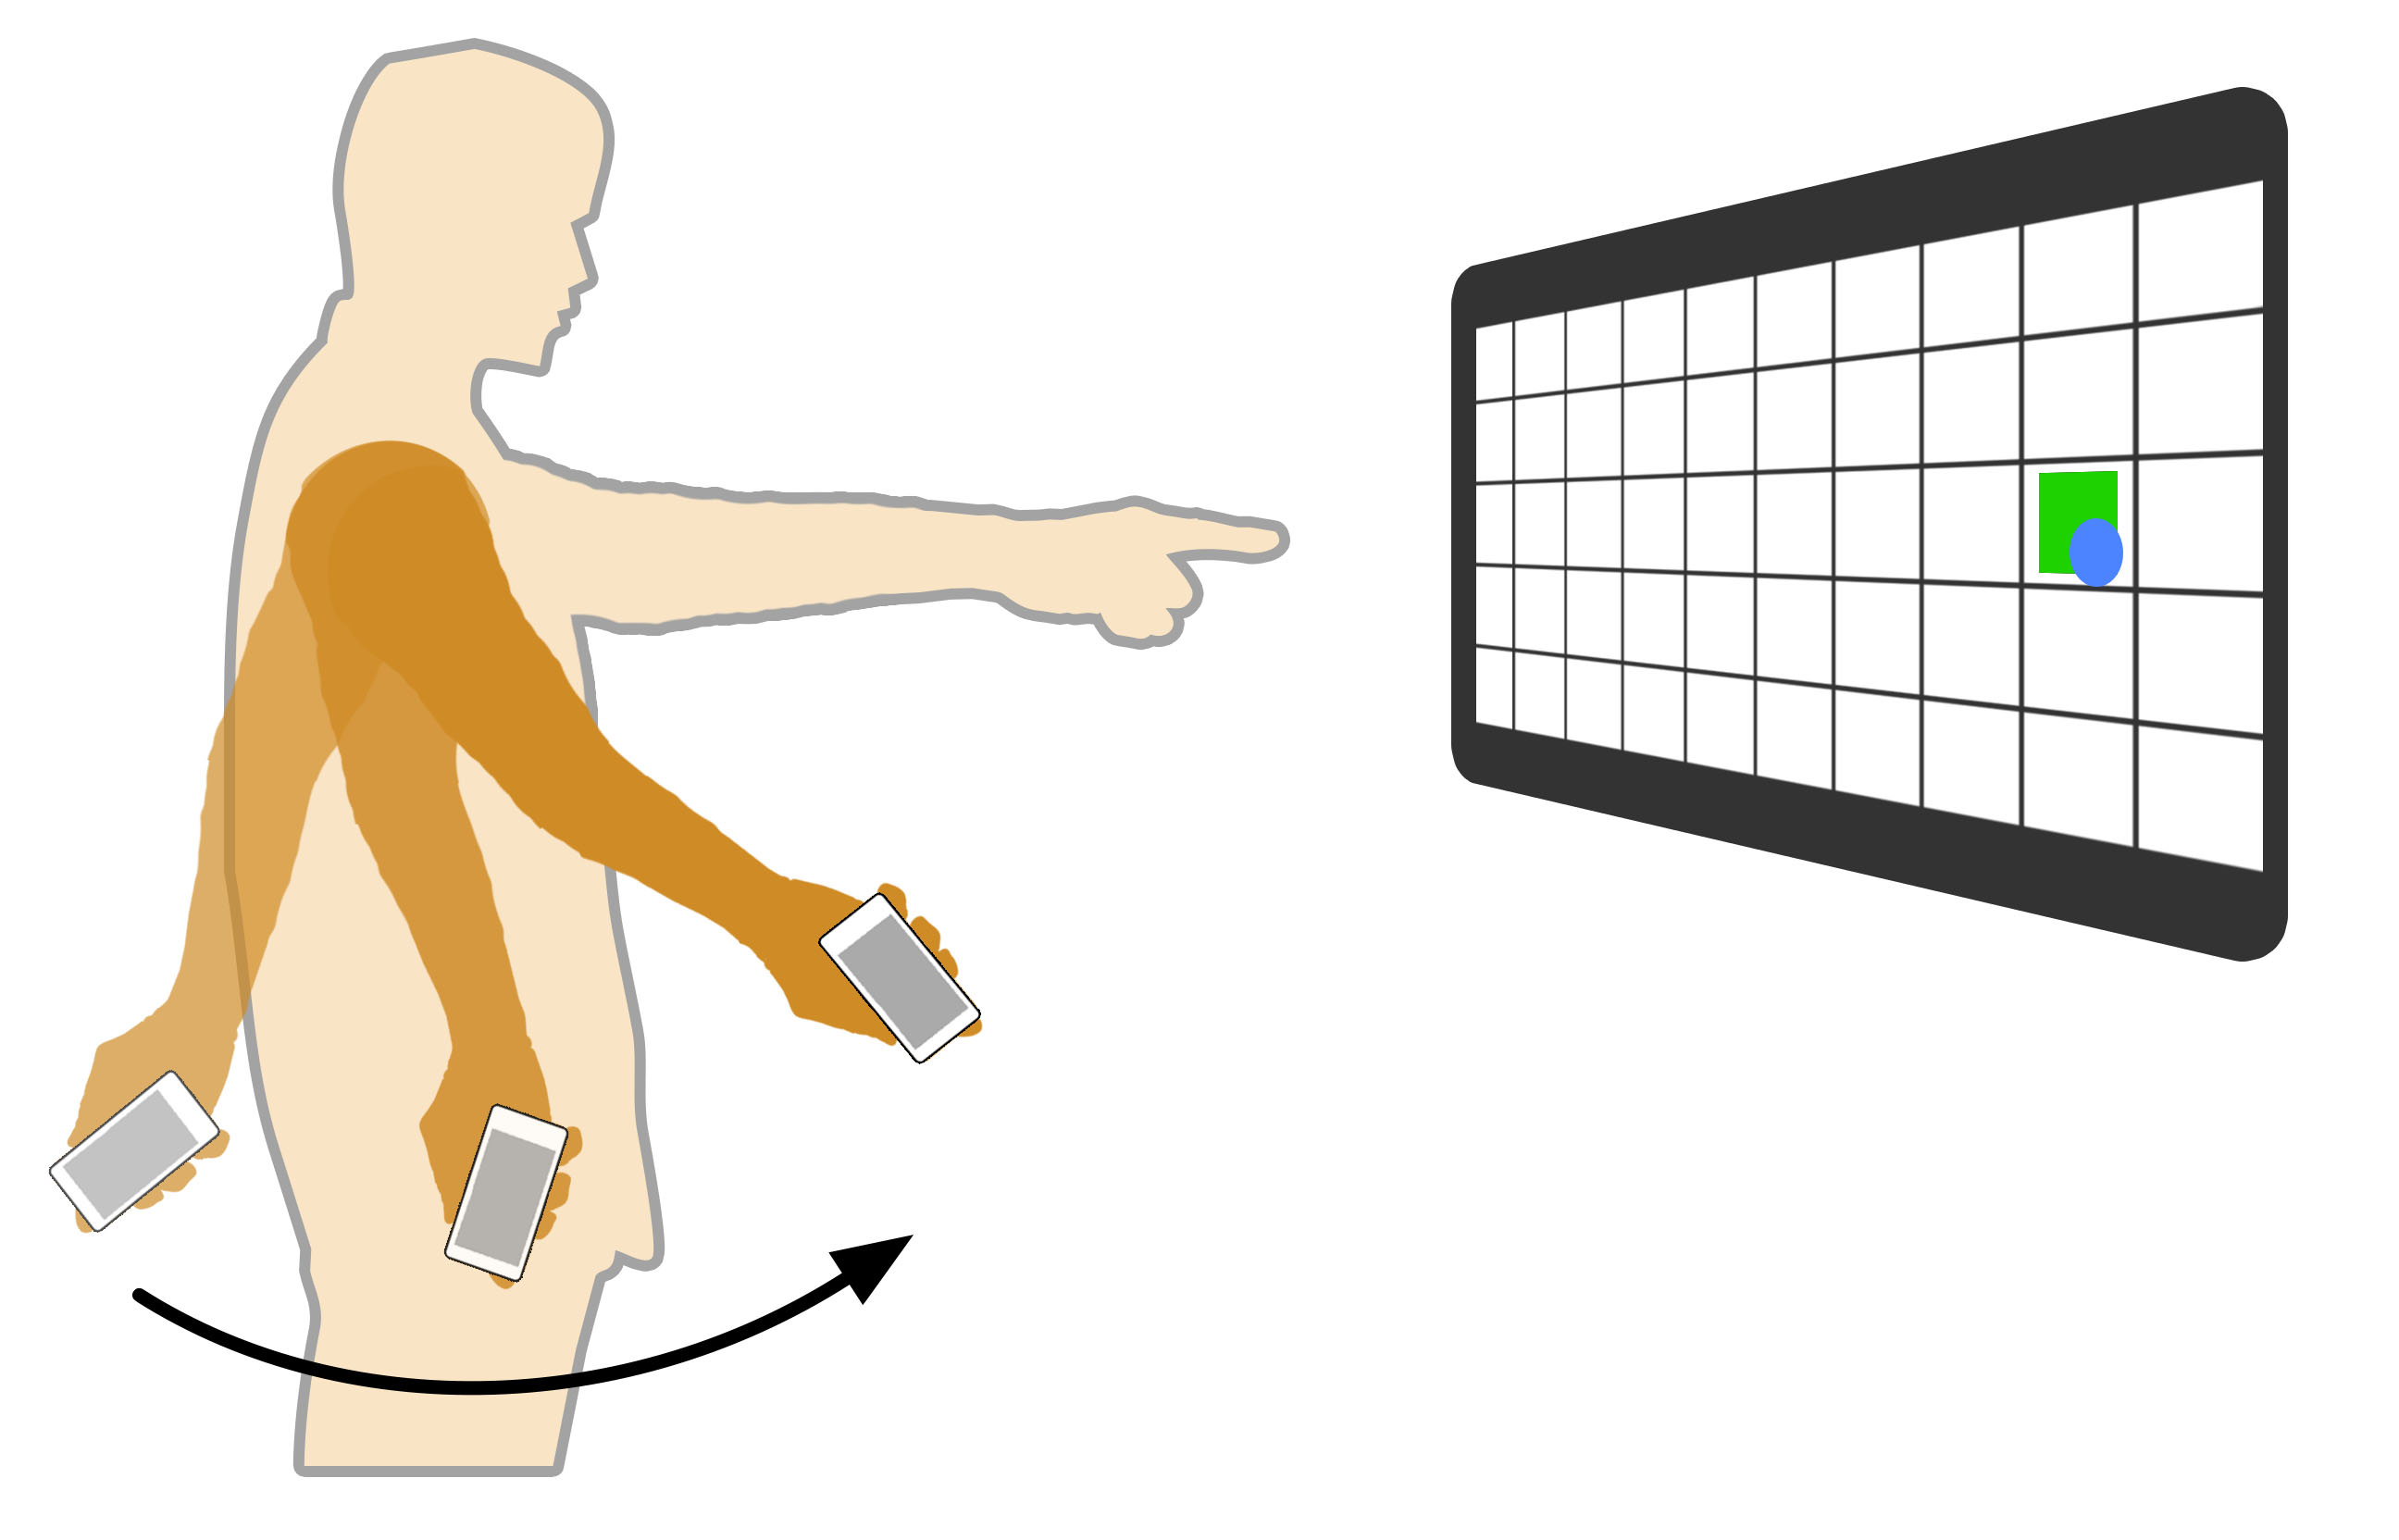
\includegraphics[width = 0.33\columnwidth]{images/techniques/throwPush3.jpg}\label{fig:throwTechniqueC}}
	\caption{\push \throw technique}
	\label{fig:throwTechnique}
\end{figure}

\subsubsection{Tilt} \label{sec:tiltTechnique}
The \tilt technique (\cref{fig:tiltTechnique}) is used by Lucero et al. in \emph{MobiComics} \cite{Lucero:2012}.
They created a system in which users would transfer objects from a large display onto their mobile devices.
The \tilt technique was chosen because it is a one handed, low complexity technique with few steps needed to activate it. 
Just like the \swipe technique it is easy, straight forward and feels natural to use. 
The \tilt technique is performed as follows:
The user first points at the target location with the phone (\cref{fig:tiltTechniqueA}).
If the user is performing a \push technique, he tilts the phone away from himself(\cref{fig:tiltTechniqueB}, \cref{fig:tiltTechniqueC}).
If he is performing a \pull technique, he does the opposite and tilts the phone towards himself. 

\begin{figure}[H]
	\subfloat[]{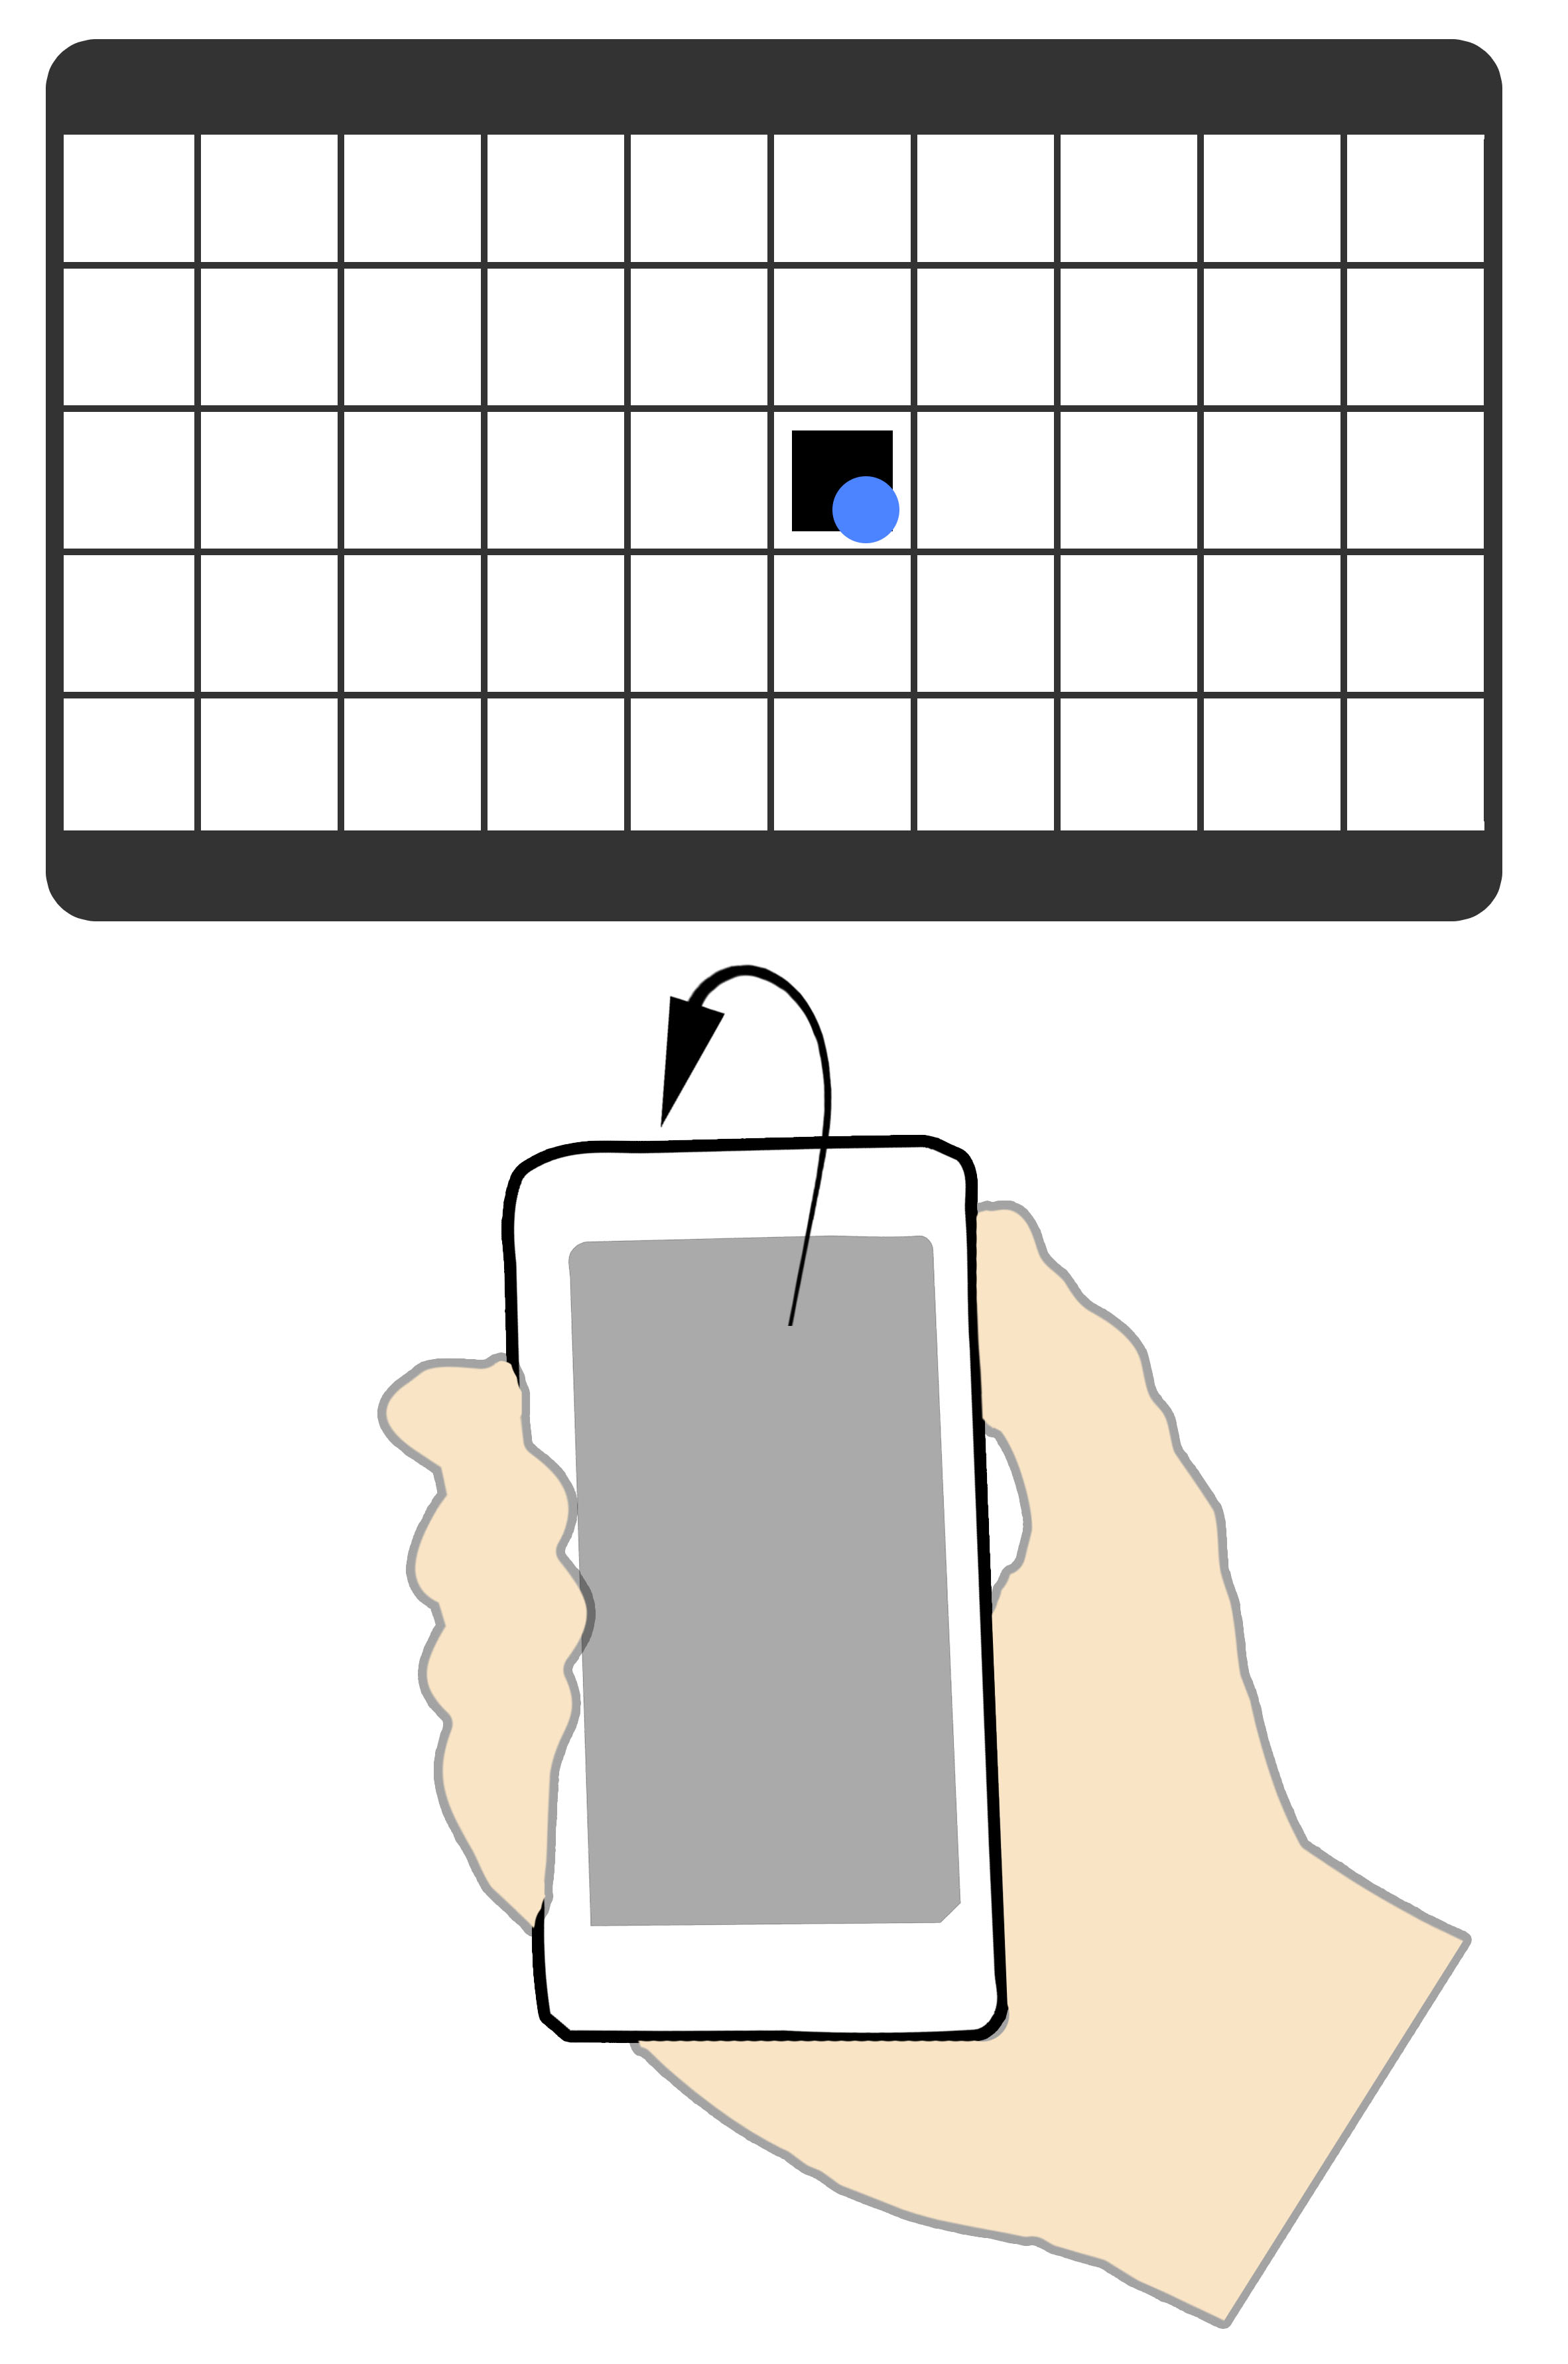
\includegraphics[width = 0.33\columnwidth]{images/techniques/tiltPush1.jpg}\label{fig:tiltTechniqueA}}
	\subfloat[]{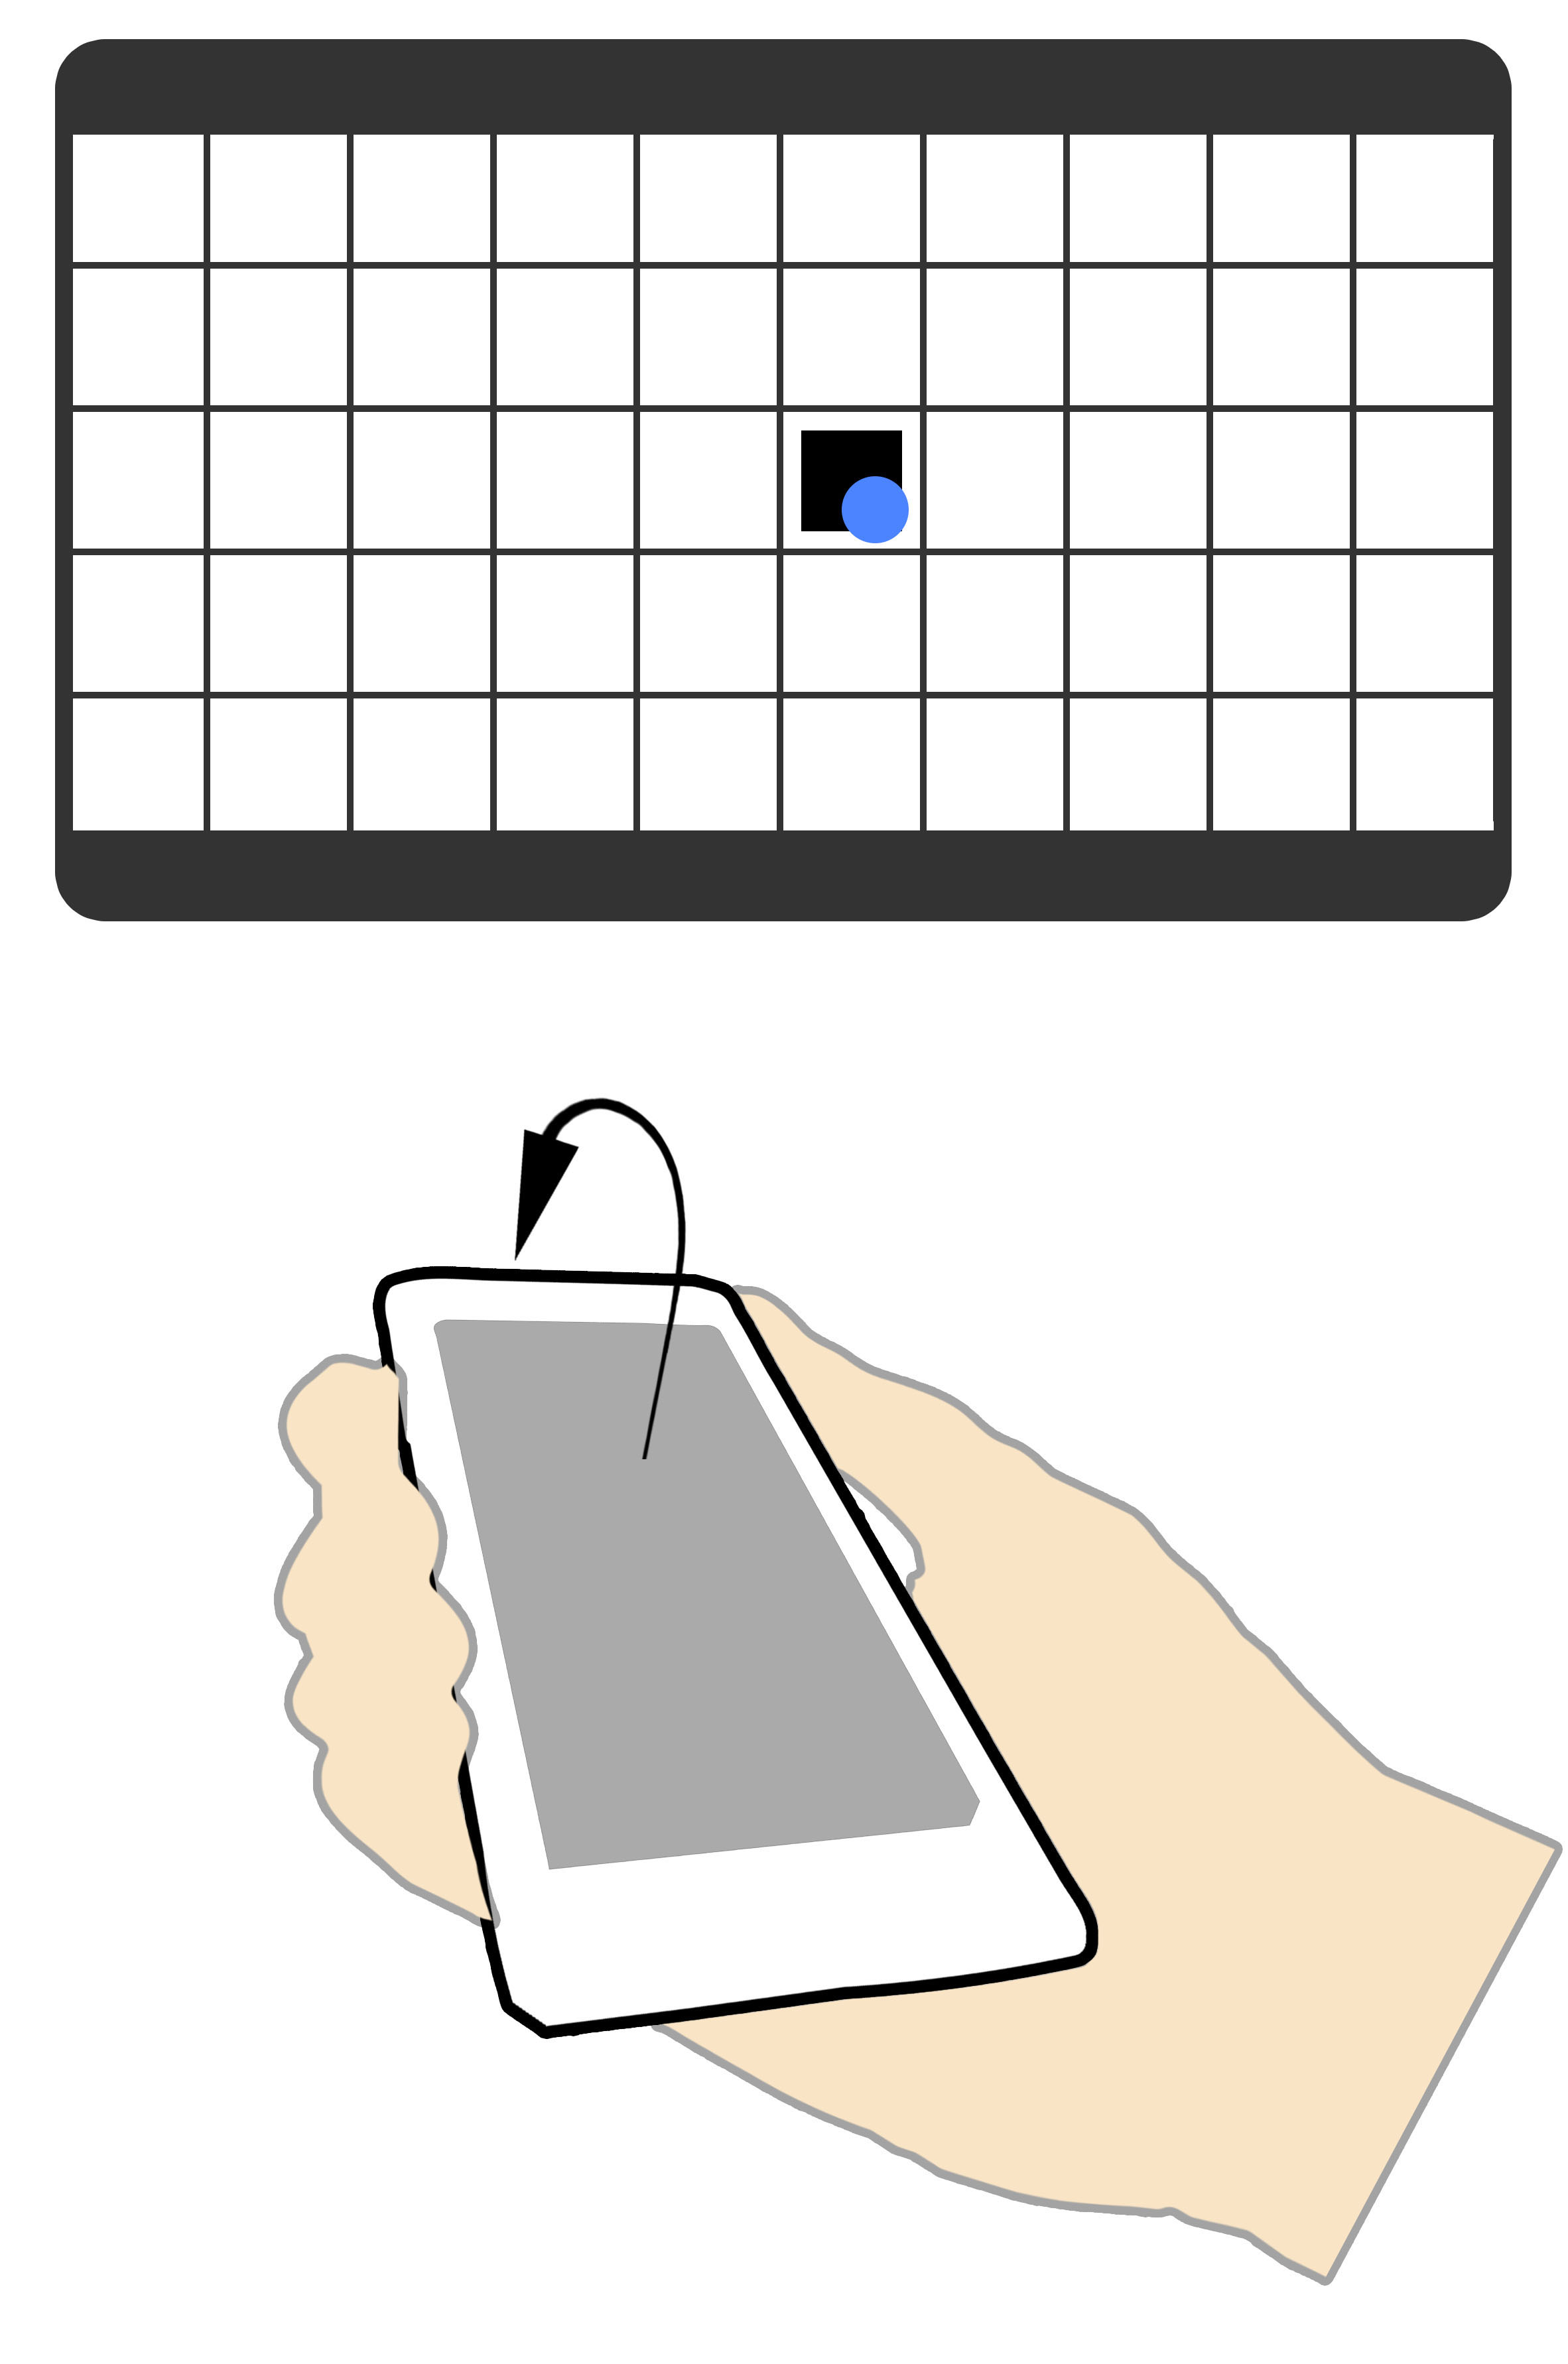
\includegraphics[width = 0.33\columnwidth]{images/techniques/tiltPush2.jpg}\label{fig:tiltTechniqueB}}
	\subfloat[]{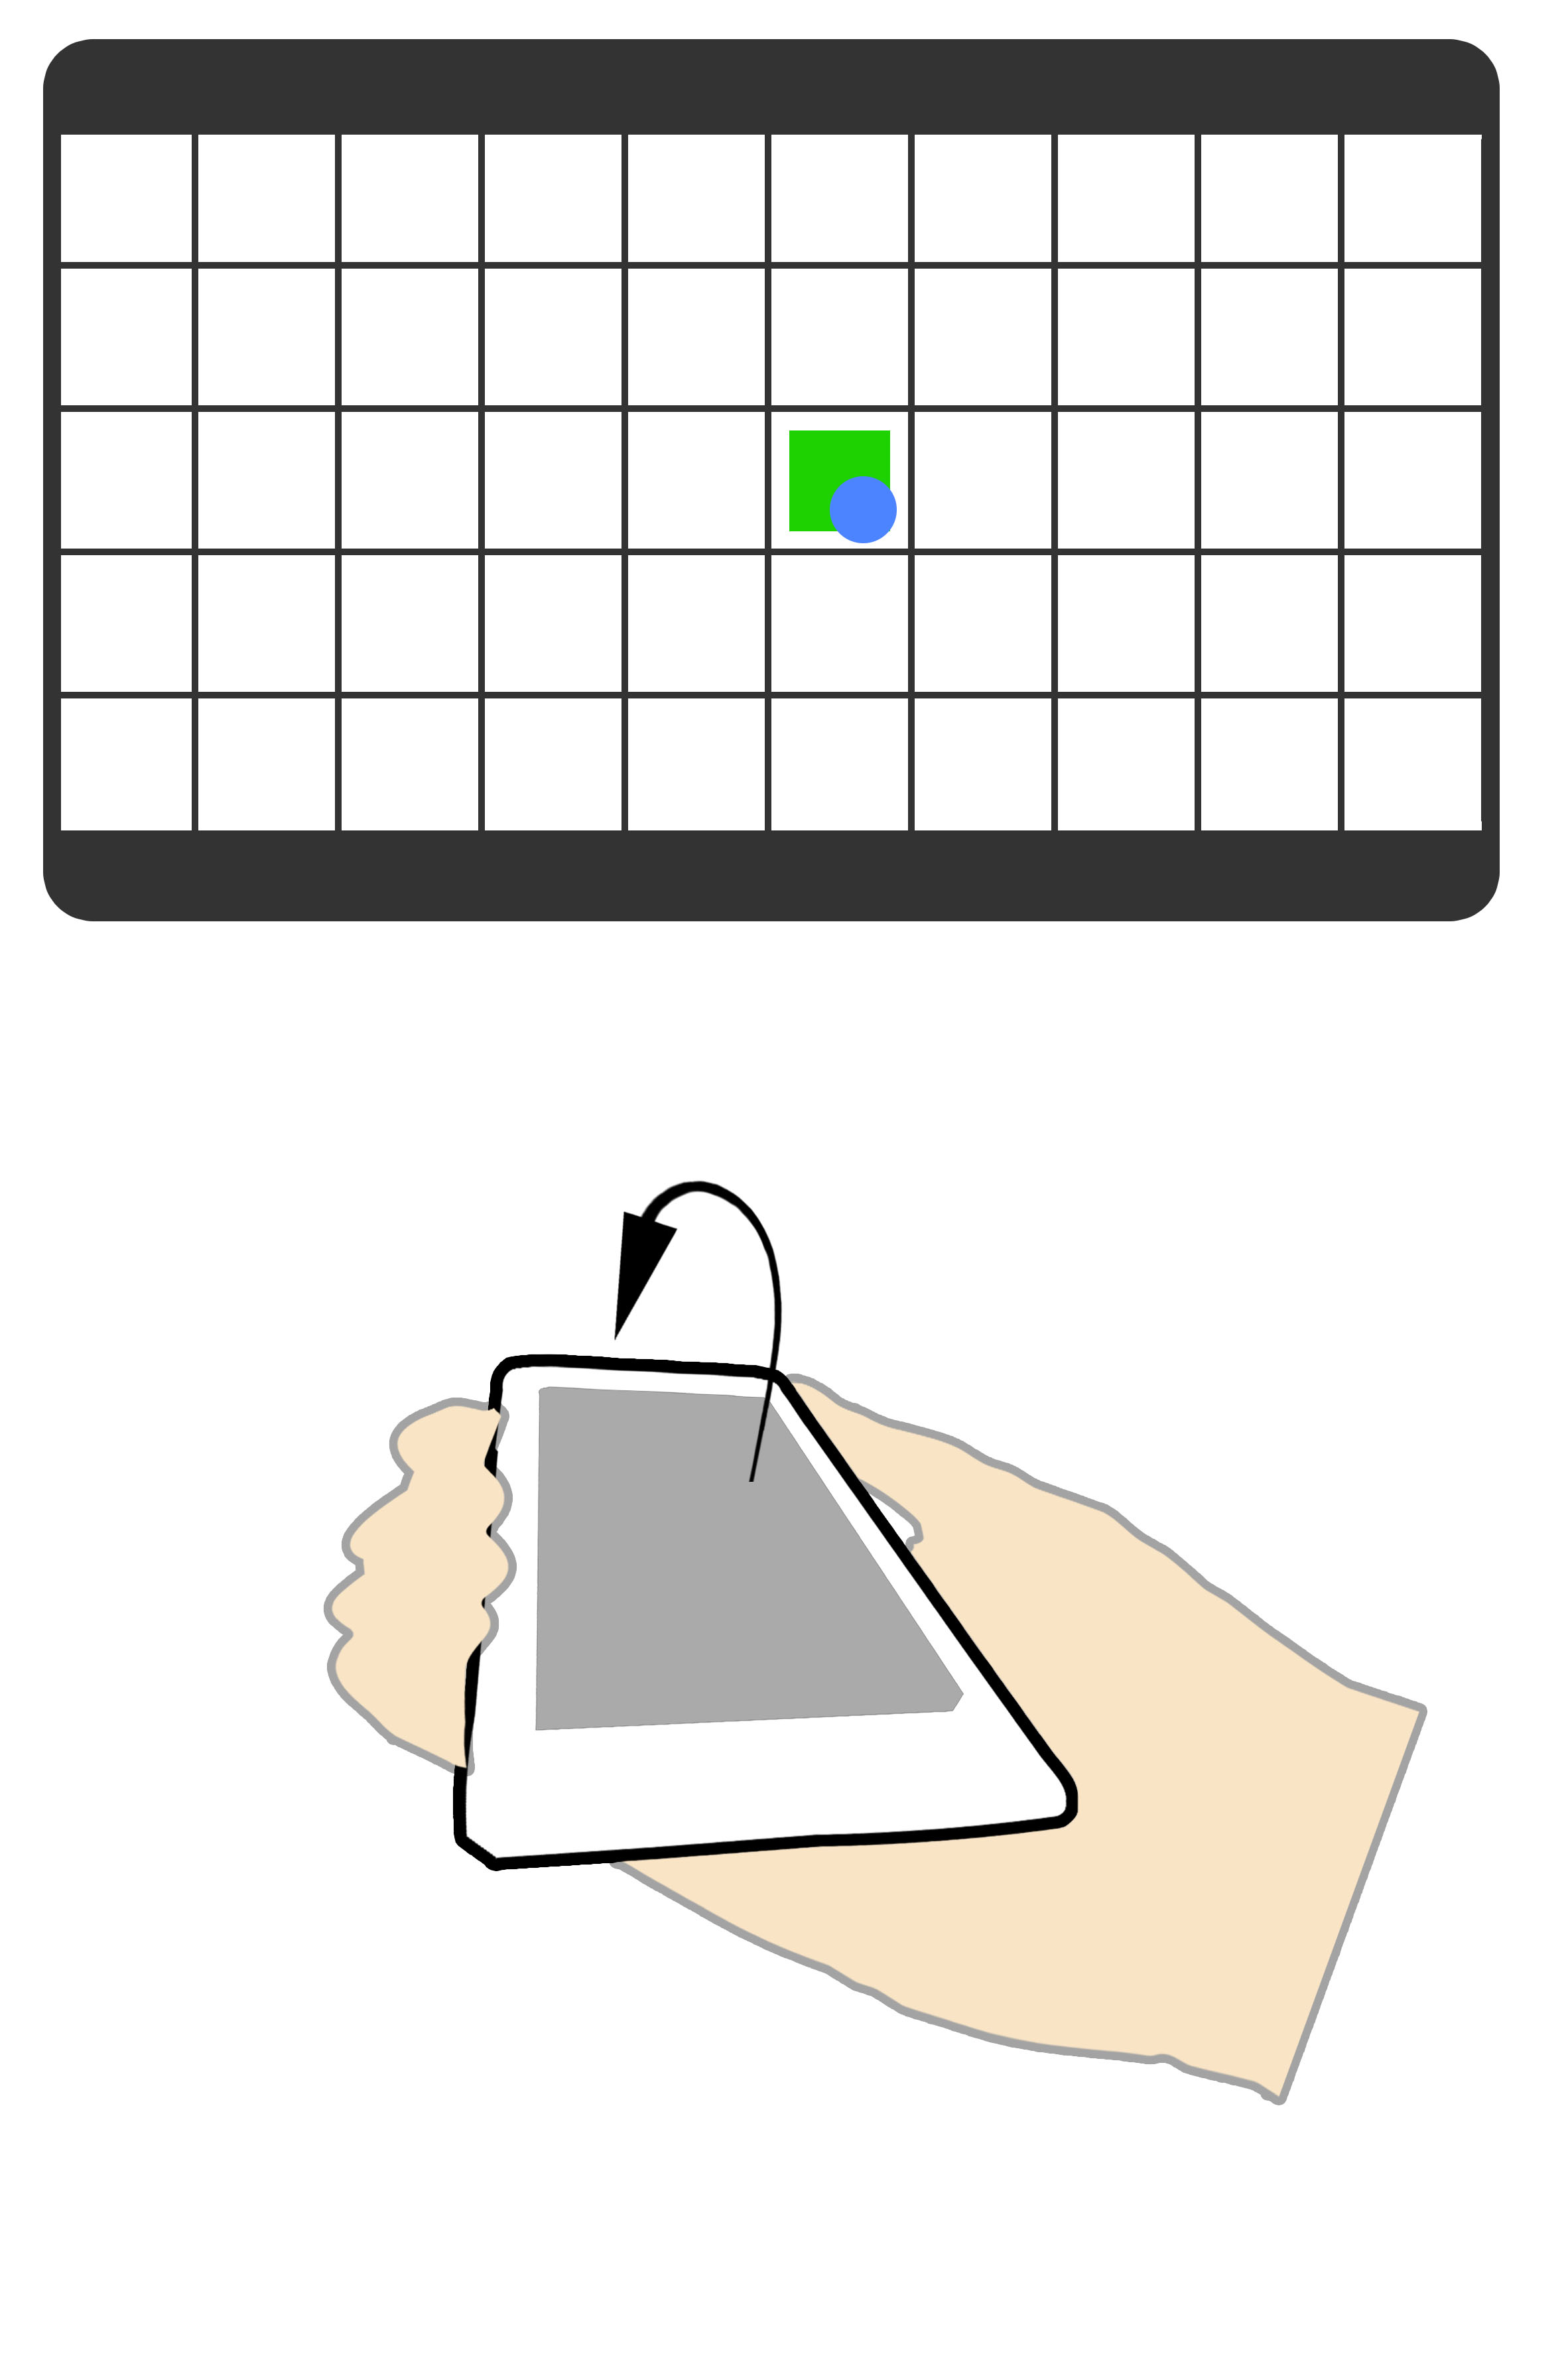
\includegraphics[width = 0.33\columnwidth]{images/techniques/tiltPush3.jpg}\label{fig:tiltTechniqueC}}
	\caption{\push \tilt technique}
	\label{fig:tiltTechnique}
\end{figure}

All techniques that were chosen have been used in other research systems to facilitate the interaction between mobile devices and large public displays.
They differ in the way they are activated as well as the number of hands that are used to perform the technique.
For our two handed techniques, we have \throw and \grab, and for one handed techniques we have \tilt and \swipe. 
Each technique also has different ways to activate it. 
The \throw and \tilt techniques require the user to move the phone, whereas the \swipe and \grab techniques require the user to touch and manipulate the screen of the device in order to activate them. 

All the techniques used in this experiment require some combination of mid-air pointing, touch gestures and phone movements to perform. 
These were all implemented using the Microsoft Kinect V2 as well as the accelerometer and touch sensors on the phone. 
The Kinect utilizes its depth camera in order to give information about a users location in physical space, allowing us to track the position of the users hands and building the techniques around that. 
The touch sensor on the phone was used in order to recognize touch and swipe gestures.
The accelerometer was used to detect significant movement on the phone and use that for the \tilt and \throw techniques. 
A detailed implementation of the system can be found in \cite{9thSemester:2015}.
